%\ihead{\headmark}
\chapter{ECG Signal and Data Processing}


\section{Devices}

Wireless sensor devices and contact-less sensor devices are the current trends in the health informatics. The recent improvements in the sensor devices made it possible for the people to bring this idea
into reality. When  medical sensor devices are combined with cloud computing, it can be thought of as a complete
solution for a health care system which not only can be used
in hospitals but also can be utilized out of the hospital when
the doctor is unreachable regardless of the patient's location.
Doctors will still be able to monitor his patient condition and
according to the patient situation they can instruct the device,
that is, attached to the patient, to take appropriate actions.
One example can be thought of as a person running somewhere and during that he/she feels some heart pain. Sensors assess the patient's condition and immediately send some notification to the doctor. After looking at the conditions, he sends back a response to the devices, which then acts according to the instruction such as, injects some medicine into the patient body. It can also be used to keep track of the patient location so, in the case of emergency, an ambulance can be instructed to go there.
Many of the sensors can be installed in the patient's surrounding, whereas,
several sensors can be wearable. These sensors can monitor
body temperature, respiration, heart rate, blood pressure, ECG, EEG, etc.
Along with sensors, it might be possible that there are several
actuators attached to the patient body which is activated by
certain events such as the rise of sugar level in blood.

Multiple contact-less sensor devices are used to implement a system for the thesis, which collects data of the user and process that in real-time. The following devices are used in the implementation:

\subsection{Magnetic Impedance Sensor}

The magnetic impedance (MI) sensor measures the small changes in electrical resistance of the chest or different regions of the body. It uses special electrodes which emit very low voltage electric current into the body. As the voltage level is very low, therefore, it does not interfere with the heart's electrical system. The MI sensor measures the resistance to the flow of current as it passes through the body via blood, as blood is a good conductor.

During systole, as the blood volume increases, impedance decreases. Similarly, during diastole, the blood volume decreases and the impedance increases.


\begin{figure}%
	\centering
	
	\subfigure[]{%
		\label{fig:ex3-e}%
		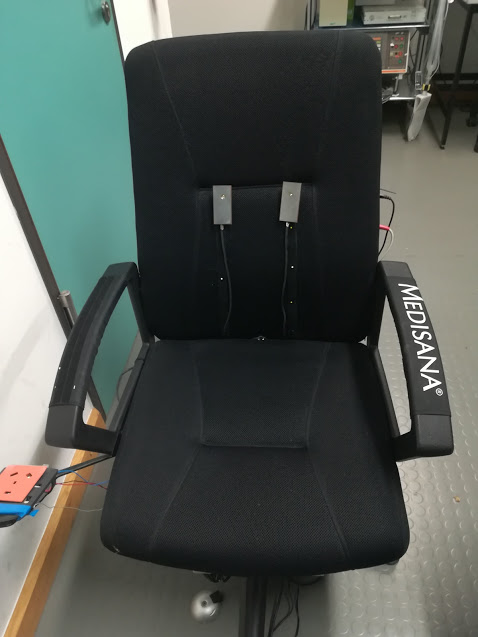
\includegraphics[height=2in]{images/ecg}}%
	\hspace{8pt}%
	\subfigure[][]{%
		\label{fig:ex3-a}%
		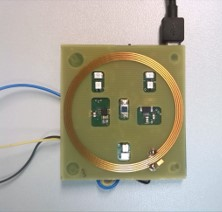
\includegraphics[height=2in]{images/mi}}%
	\hspace{8pt}%
	\subfigure[][]{%
		\label{fig:ex3-b}%
		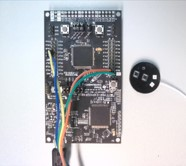
\includegraphics[height=2in]{images/ppg}} \\
	\subfigure[][]{%
		\label{fig:ex3-c}%
		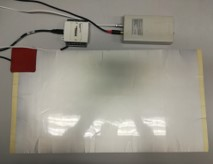
\includegraphics[height=2in]{images/bcg}}%
	\hspace{8pt}%
	\subfigure[][]{%
		\label{fig:ex3-d}%
		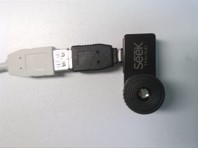
\includegraphics[height=2in]{images/tc}}%
	\caption[A set of sensor devices.]{A set of sensor devices:
		\subref{fig:ex3-e} an ECG sensor;
		\subref{fig:ex3-a} a MI sensor;
		\subref{fig:ex3-b} a PPG sensor;
		\subref{fig:ex3-c} a BCG sensor; and,
		\subref{fig:ex3-d} a thermal camera.}%
	\label{fig:ex3}%
\end{figure}



The MI sensor provides a data packet of 42 bytes, which splits into the attributes shown in table \ref{tab:att_mi}. The byte identifier of the sensor can be seen in the table \ref{tab:bi_mi}.

There is an exception in the data packet when it contains 0x8101 or 0x8102. In this case, the size of the data packet may vary according to the number of count of the corresponding bytes. Moreover, the data packet should be examined and if it contains the corresponding bytes, the data packet should be modified and the bytes 0x8101 should be replaced with 0x81 and 0x8102 should be replaced with 0x82. This modification has been done in order to differentiate it with the header and data packet identifier as they have the same value.


\renewcommand{\arraystretch}{2}
\begin{table}
	\caption{Attributes of MI s
		ensor.} \label{tab:att_mi}
	
	\begin{center}
		\begin{tabular}{ | l | r | }
			\hline
			\textbf{Attributes} & \textbf{Size (Bytes)} \\ \hline
			MI\_RAW  & 4 \\ \hline
			MI  & 4  \\ \hline
			RED\_RAW  & 4  \\ \hline
			ECG\_RAW  & 4  \\ \hline
			IR\_RAW  & 4  \\ \hline
			RED\_AVG  & 4  \\ \hline
			ECG\_AVG  & 4  \\ \hline
			IR\_AVG  & 4  \\ \hline
			ACC\_X  & 2  \\ \hline
			ACC\_Z  & 2  \\ \hline
			ECG\_REF  & 2  \\ \hline
			RESP\_REF  & 2  \\ \hline
			BATTERY  & 2  \\ \hline
		\end{tabular}
	\end{center}
	
\end{table}


\renewcommand{\arraystretch}{2}
\begin{table}
	\caption{Byte identifiers for the MI sensor.} \label{tab:bi_mi}
	
	\begin{center}
		\begin{tabular}{ | l | r | }
			\hline
			\textbf{2-Byte Identifier} & \textbf{Description} \\ \hline
			0x81  & Header \\ \hline
			0x82  & Data Packet  \\ \hline
		\end{tabular}
	\end{center}
	
\end{table}

\subsection{Photoplethysmogram Sensor}
The photoplethysmogram (PPG) sensor is used to measures the variations in blood flow in the body with each heartbeat. A PPG sensor uses a light source to illuminate the blood and a photo-detector to measures the variations in the light intensity associated with changes in the blood volume. The decrease in light intensity indicates the increase in blood volume and increase in light intensity indicates the decrease in blood volume.

The sensor provides the PPG signal with 4 different channels, a temperature, which is measured in Celsius and accelerometer coordinates. The size of the data changes according to the attributes which can be seen in the table \ref{tab:att_ppg}. The frequency of the data packets changes according to the attributes. The temperature value is sent every one second, whereas, the frequency rate of PPG channels is 100 samples per second. Similarly, for the accelerometer coordinates, the data rate is 50 samples per second.

% Please add the following required packages to your document preamble:
% \usepackage{multirow}
\begin{table}[]
	\centering
	\caption{Attributes of PPG Sensor.}
	\label{tab:att_ppg}
	\begin{tabular}{|l|l|l|l|}
		\hline
		\textbf{2-Byte Identifier} & \textbf{Attributes} & \textbf{Size (Bytes)} & \textbf{Data} \\ \hline
		\multirow{4}{*}{} 0x0050 & \multirow{4}{*}{} ppg (8 Bytes) & 2 & Channel 1 \\ \cline{3-4} 
		&                   & 2 & Channel 2 \\ \cline{3-4} 
		&                   & 2 & Channel 3 \\ \cline{3-4} 
		&                   & 2 &  Channel 4 \\ \hline
		0x0054 & Temperature (2 Bytes) & 2 & Temperature \\ \hline
		\multirow{3}{*}{} & \multirow{3}{*}{} & 2 & X Coordinate \\ \cline{3-4} 
		0x0041 & Accelerometer coordinates (6 Bytes) & 2 & Y Coordinate \\ \cline{3-4} 
		&  & 2 & Z Coordinate \\ \hline
	\end{tabular}
\end{table}


\subsection{ECG Sensor}
As described in section \ref{the_electrocardiogram}, the ECG signal is usually collected by placing electrodes directly on the body but it has several disadvantages as well, which is described in section \ref{electrodes_disadv}. Therefore, non-contact capacitive electrodes have been used to collect the ECG signals of the person. Unlike traditional electrodes, which rely on galvanic contact, the capacitive electrodes are insulated from skin using a dielectric material, such as, air gap, clothes, etc \cite{bouchard2017smart}. The ECG signal propagates via skin to the dielectric material and then to the electrodes through a capacitive coupling. The major drawback of this approach is that it is very sensitive to body motion.

\subsection{Ballistocardiogram Sensor}
The ballistocardiogram (BCG) sensor measures the ballistic forces associated with cardiac contraction and ejection of blood. These ballistic forces are mainly measures by the electromechanical film (EMFi) sensor which converts the mechanical energy into the electrical signal and vice versa. Most of the time, the EMFi sensing device is placed on a chair or bed, which measures the pressure associated with the cardiac activity.

\subsection{Thermal Camera}
A thermal camera is also used to measures the temperature of the person. A thermal seek camera is used for the implementation which captures the thermo temperature images, from which then the temperature is calculated.

\section{ECG Signal Processing}
QRS complex detection is the basis for processing ECG signal. Regardless of what application is required, the accurate detection of QRS complex is a pre-requisite for feature extraction. In order to detect the QRS complex accurately, it is necessary to detect the R-peak position correctly. Once the QRS complex is identified, further examination of the signal can be performed such as heart rate, arrhythmias, classification of ECG signal, ST segment etc. Moreover, P and T waves can also be extracted.

The ``QRS Complex'' is the combination of Q, R and S waves and it represents the contraction of the ventricles. It plays a significant role in the detection of cardiac arrhythmias.

Many methods have already been proposed for the detection of QRS complex. These methods fall into 3 categories \cite{5639905}.

\begin{enumerate}
	\item Filter Method
	\item Artificial Intelligence Method
	\item Wavelet transform Method
\end{enumerate}

\subsection{Filter Method}
The filter method uses bandpass filter to filter the ECG signal \cite{4122029}\cite{554762}. In this method, a QRS complex is intensified by suppressing the P and T wave. This method is generally very quick and takes less time to implement. But the major drawback of this method is that the frequency band of QRS complex and of noise overlapping, affect its performance.

\subsection{Artificial Intelligence Method}
The detection of QRS complex using this method is fast, accurate and more robust, but in reality, it is very time-consuming and difficult to implement \cite{126604}\cite{PIETKA1991139}\cite{58593}. Therefore, this method is not very popular and not widely used as compared to the other methods.

\subsection{Wavelet Transform Method}
Wavelet transform method becomes very popular in detecting the QRS complex. It is based on time-frequency analysis. It is very efficient and takes less to implement. Many people have already used wavelet transform for detecting the QRS complex. Yazhu Qiu \cite{PMID:17228741} used Mexican-hat wavelet to detect ECG signal. In the proposed method, although the processing was fast, but it sometimes didn't detect the onset and offset of QRS complex accurately. Nevertheless, it is considered as simple, faster and easier to implement comparatively.


In the implementation of this thesis, the wavelet transform method has been used to extract the ECG signal features.

\section{Wavelet Transform}
Transformation is applied to signal in order to get further information about the signal which is not easily available in the raw signal. Most of the time, signals are generally represented in the time domain, but in many cases, the important information is hidden in the frequency domain of the signal. Fourier transform is a tool which allows viewing the frequency components of the signal. But the major drawback of this transformation is that a signal cannot be viewed in both time and frequency domain at the same time. Thus, it makes hard to distinguish which frequency components exist at any instance of time. Therefore, a tool was required which helps to view signal in both domains.

A wavelet transform is a very useful tool for analyzing the signal simultaneously in both time and frequency domain \cite{addison2017illustrated}. It uses a little wavelike functions known as \textbf{\textit{wavelets}}. Wavelets are used to transform a signal into another representation where signal information can be viewed in a more useful form.

Generally, there are two operations involved with wavelet. Either they can be stretched or squeezed or can be translated to other locations on the signal and if the wavelet matches the shape of the signal at specific location or scale, it produces a large transform value. And similarly, if the signal and the wavelet do not correlate, it produces a low transformed value. There is a single function called "mother wavelet" which is stretched or translated to produce a family of basis functions known as "daughter wavelets". It is defined as:

\begin{equation} \label{eqn_mother_wavelet}
{\Psi_{a,b}(t) = \frac{1}{\sqrt{|a|}}\Psi \bigg(\frac{t-b}{a}\bigg),\quad a, b \in \mathbb{R}, a \neq 0}
\end{equation}

where \textit{a} is the scaling parameter which measures the degree of the scale, and \textit{b} is the translation parameter which measures the time location of the wavelet. If |\textit{a}| < 1, then it mainly corresponds to higher frequencies. And on the other hand, if |\textit{a}| > 1, it corresponds to lower frequencies. It is important to note here that the variation in time and frequency scale of the wavelet is supervised by the Heisenberg uncertainty principle. At large scale, the time domain is not very clear, whereas, in the frequency domain is much finer. As the scale decreases, the frequency domain becomes worse, whereas, time domain becomes finer.

The wavelet transform is defined as:

\begin{equation} \label{eqn_wavelet_transform}
{X_{W}(a, b) = \frac{1}{\sqrt{|a|}} \int_{-\infty}^\infty h*\bigg(\frac{t-b}{a}\bigg)x(t) \mathrm{d}x}
\end{equation}


Biorthogonal Spline wavelet has been used for the detection of ECG signal characteristics \cite{zheng2008detection} \cite{pan2010detection} \cite{meena2014comparison}. This approach is based on the modulus maxima of zero point to detect the singular point. 


For multi-resolution decomposition of signals, a dyadic DWT (discrete wavelet transform) is used where all bandpass filters have different frequency resolution. This is done by first using low-pass and high-pass filters to split the signal into low and high-frequency components.

\section{Biorthogonal Spline Wavelet Filter Construction}
Let say, ${H_{0}(z)}$ and ${H_{1}(z)}$ are low-pass filters in the analysis filter bank (decomposition) and ${G_{0}(z)}$, ${G_{1}(z)}$ are high-pass filters in the synthesis filter bank (reconstruction) \cite{wang2001using}, as can be seen in the figure \ref{fig:2_channel_filter_bank}. After passing the input signal $X[n]$ from the filters, the resulting signal is first down-sampled by 2 and then up-sampled by 2  respectively, producing the final output signal $Y[n]$. It is worth to note here that $Y[n]$ is the reconstructed signal. 



%\begin{figure}[h] for figure at the place, where we put the picture.
\begin{figure}
	\centering
	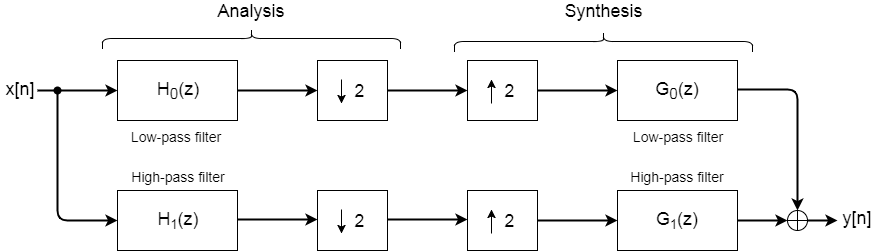
\includegraphics[width=160mm]{images/2_channel_filter_bank}
	\caption{Two-channel filter bank}
	\label{fig:2_channel_filter_bank}
\end{figure}



The idea is to determine $H_0$, $H_1$, $G_0$ and $G_1$ such that, $Y[n]$ is just a delayed version of input signal $X[n]$. This is called as perfect reconstruction filter bank. A perfect reconstruction filter bank is also known as ``biorthogonal`` and the associated filters as biorthogonal filters. 

After passing the input signal from the channel 1, it will produce:

\begin{equation} \label{eqn_wavelet_transform}
{Y_{0}(z) = \frac{1}{2}G_{0}(z)[H_{0}(z)X(z) + H_{0}(-z)X(-z)]}
\end{equation}

Similarly, for the 2nd channel, it will produce:


\begin{equation} \label{eqn_wavelet_transform}
{Y_{1}(z) = \frac{1}{2}G_{1}(z)[H_{1}(z)X(z) + H_{1}(-z)X(-z)]}
\end{equation}

Adding the output of these 2 channels will produce the final output.



\begin{equation} \label{eq1}
\begin{split}
Y(z)  &= Y_{0}(z) + Y_{1}(z) \\
&= \frac{1}{2}G_{0}(z)[H_{0}(z)X(z) + H_{0}(-z)X(-z)] + \frac{1}{2}G_{1}(z)[H_{1}(z)X(z) + H_{1}(-z)X(-z)]
\end{split}
\end{equation}


Arranging $Y(z)$ in such a way so that, one part should depends on $X(z)$ and the other part on $X(-z)$. We get,

\begin{equation} \label{eqn_wavelet_transform}
{Y(z) = \frac{1}{2}[G_{0}(z)H_{0}(z) + G_{1}(z)H_{1}(z)]X(z) + \frac{1}{2}[G_{0}(z)H_{0}(-z) + G_{1}(z)H_{1}(-z)]X(-z)}
\end{equation}

The important thing to note here is that $X(-z)$ is the aliasing part, and $X(z)$ is the distortion part.

%In order to satisfy the condition, $Y(n) = X(n-k)$ ($Y(z) = X(z)z^{-k}$) i.e., %the output signal $Y(z)$ to be some sort of delayed version of input signal, we %need to satisfy 2 conditions:

\subsection{Design of Biorthogonal Spline Wavelet Filter}

The perfect reconstruction for filter bank can be achieved if the following two conditions are satisfied.

\begin{enumerate}
	\item No aliasing: 
	\begin{equation} 
	{G_{0}(z)H_{0}(-z) + G_{1}(z)H_{1}(-z)]X(-z) = 0}
	\end{equation}
	\item No distortion:
	\begin{equation} 
	{G_{0}(z)H_{0}(z) + G_{1}(z)H_{1}(z) = mz^{-k}}
	\end{equation}
\end{enumerate}


where $m$ is constant and $k$ is a time delay.

In order to satisfy condition 1 i.e., to get rid of aliasing, one can do:

\begin{align}
	\label{eqn:antialiasing_cdn}
	\begin{split}
		G_0(z) &=  H_1(-z), \\ 
		G_1(z) &=  -H_0(-z)
	\end{split}
\end{align}


So now, we only need to find two filters values instead of four. Lets assume that,

\begin{equation}\label{eqn:p0} 
{P_0(z)=G_{0}(z)H_{0}(z)}
\end{equation}

From equation \ref{eqn:antialiasing_cdn} and \ref{eqn:p0}, we can deduce:

\begin{equation} 
{G_{1}(z)H_{1}(z) = -H_{0}(-z)G_{0}(-z) = -P_0(-z)}
\end{equation}

After getting these values, the condition 2 (no distortion) can be re-written as:

\begin{equation}\label{eqn:updated_no_distortion} 
{P_0(z) - P_0(-z) =  mz^{-k}}
\end{equation}

In the above equation, only one filter value is required i.e., $P_0(z)$ (also called half-band filter). The perfect reconstruction conditions naturally imply that both analysis and the synthesis filters are biorthogonal to each other, i.e., a biorthogonal filter bank makes sure that synthesis filter bank is the inverse of analysis filter bank.


\subsection{Steps for Designing FIR Filter Bank}
The steps for designing FIR filter bank can be summarized as:

\begin{enumerate}
	\item Design a low-pass filter for $P_0(z)$ which satisfy the equation \ref{eqn:updated_no_distortion}. One option is to use Daubechies function to find the value for $P_0(z)$: \\ 
	\begin{equation}\label{eqn:updated_no_distortion} 
	{P_0(z) = (1 + z^{-1})^{2p}Q(z)}
	\end{equation} \\
	where $p$ can be any integer and $Q(z)$ be a polynomial of degree $(2p-2)$.
	\item Factorize $P_0(z)$ to get the values for $G_0(z)$ and $H_0(z)$.
	\item Find the filter coefficients for high-pass filters using the equations \ref{eqn:antialiasing_cdn}. 
\end{enumerate}


Lets assume that, $P=2$ and and $Q(z)$ be a quadratic polynomial $(a + bz^{-1} + cz^{-2})$. Substituting these values in equation \ref{eqn:updated_no_distortion} will produce a polynomial of degree $z$:

\begin{equation} 
{P_0(z) = (1 + z^{-1})^4(a + bz^{-1} + cz^{-2})}
\end{equation}

Substituting $a = c = - \frac{1}{16}, b= 4$, we get:

\begin{equation} 
{P_0(z) = \frac{(1 + z^{-1})^4(-1 + 4z^{-1} + z^{-2})}{16}}
\end{equation}

Factorizing $P_0(z)$ to get $H_0(z)$ and $G_0(z)$. Lets say we get:

\begin{equation} \label{eq1}
\begin{split}
H_0(z) & = \frac{(1 + z^{-1})^3}{4} \\
& = \frac{(1 + 3z^{-1} + 3z^{-2} + z^{-3})}{4}
\end{split}
\end{equation}


and


\begin{equation} \label{eq1}
\begin{split}
G_0(z) & = \frac{(1 + z^{-1})(-1 + 4z^{-1} + z^{-2})}{4} \\
& = \frac{(-1 + 3z^{-1} + 3z^{-2} - z^{-3})}{4}
\end{split}
\end{equation}


Then by equation \ref{eqn:updated_no_distortion}, we have:


\begin{equation} \label{eq1}
\begin{split}
H_1(z) = G_0(-z) \\
& = \frac{(-1 - 3z^{-1} + 3z^{-2} + z^{-3})}{4}
\end{split}
\end{equation}

and

\begin{equation} \label{eq1}
\begin{split}
G_1(z) = -H_0(-z) \\
& = \frac{(-1 + 3z^{-1} _ 3z^{-2} + z^{-3})}{4}
\end{split}
\end{equation}

Therefore, the filter coefficients are:

\begin{equation}
\label{eqn:filters}
\begin{aligned}
h_0(0) & =  \quad \frac{1}{4}    & \quad &\quad  h_0(1) &= \quad \frac{3}{4} \\
h_0(2) & =  \quad \frac{3}{4}    & \quad &\quad   h_0(3) &= \quad \frac{1}{4} \\[1ex]
h_1(0) & =  \quad \frac{- 1}{4}  & \quad &\quad   h_1(1) &= \quad \frac{-3}{4} \\
h_1(2) & =  \quad \frac{3}{4}    & \quad &\quad   h_1(3) &= \quad \frac{1}{4} \\[1ex]
g_0(0) & =  \quad \frac{-1}{4}   & \quad &\quad   g_0(1) &= \quad \frac{3}{4} \\
g_0(2) & =  \quad \frac{3}{4}    & \quad &\quad   g_0(3) &= \quad \frac{-1}{4} \\[1ex]
g_1(0) & =  \quad \frac{-1}{4}   & \quad &\quad   g_1(1) &= \quad \frac{3}{4} \\
g_1(2) & =  \quad \frac{-3}{4}   & \quad &\quad   g_1(3) &= \quad \frac{1}{4}
\end{aligned}
\end{equation}




\section{Mallat's Algorithm}
The binary wavelet transform or dyadic wavelet transform of a signal $f(n)$ can be calculated by using Mallat algorithm \cite{119727} as follows:

\begin{equation} 
{ s_{2^j}f(n) = \sum h_ks_{2^{j-1}}f(n - 2^{j-1}k),   }
\end{equation}

\begin{equation} 
{ w_{2^j}f(n) = \sum g_ks_{2^{j-1}}f(n - 2^{j-1}k).   }
\end{equation}

where, $s_{2^0}f(n)$ is the original signal to be processed. In our case, it is ECG signal. $w_{2^j}f(n)$ is the wavelet coefficient i.e., the dyadic wavelet transform of the signal and $s_{2^j}f(n)$ is the approximation coefficient for the scale j. $h_k$ and $g_k$ are the coefficients of a low-pass filter and high-pass filter respectively which are defined in the equation \ref{eqn:filters}. The signal is decomposed into several frequency bands at certain scale j and then the frequency bands which have noises, are set to zero. And by using the synthesis filters, the de-noised signal can be reconstructed.



%\section{Singular Point Detection of QRS Complex Based on Wavelet Transform}
\section{Using Wavelet Transform to Identify Singular Point of QRS Complex}

\subsection{Feature Extraction Using Wavelets}
Most of the time, the important information of signal resides on the irregularities and singularities of the signal and wavelets can be used to extract that information. When the filter bank and wavelets are chosen appropriately, the wavelets are able to capture the irregularities and singularities of the signal. Mathematically, the local singularity of a signal is measured using Lipschitz exponent, the inflection points of signal $f(n)$ appear as extrema at $\frac{df(t)}{dt}$ and as zero crossing points at $\frac{d^2f(t)}{dt}$. Therefore, Mallat has suggested using a wavelet which is the first derivative of a scaling function.

\subsection{Lipschitz Exponent}
The functions which are infinitely differentiable are described as smooth or with no singularity \cite{xing2013unifying}. If at some point, the function has noncontinuous derivative, then the point is known as the singular point. The Lipschitz exponent is a good application to measure the singularity of the point.

\subsection{Relationship between Lipschitz Exponent and Modulus Maximum}
Mallat has shown in his paper \cite{119727} that, all signals and noise in there may be completely represented by their singularities and singularities are generally referred in terms of Lipschitz exponents. If a signal is $n$ times differentiable at time $t_0$, then its nth derivative is singular and it will be described as Lipschitz $\alpha$ where $\alpha > n$. If a signal is continuously differentiable at time $t_0$, then it is non-singular and has Lipschitz exponent 1.

Signals can have negative Lipschitz exponent as well. For example, many signals have singularities with positive Lipschitz exponents whereas, noise has a negative Lipschitz exponent. Therefore, having this mind, it makes it possible to separate a signal from noise if the singularities of noise can be detected and separated.

Generally, it is known that the singularity of a signal is directly proportional to the Lipschitz exponent. Therefore, as the transform scale increases, the wavelet transform modulus maxima will also get increases (Lipschitz exponent > 0) and similarly, it will decreases when Lipschitz exponent < 0. It can be seen that R wave in the original ECG signal appears as a pair of positive and negative extreme in the waveform which resulted after the decomposition of a wavelet transform.

\section{Dataset}

The MIT-BIH Arrhythmia dataset is used for the implementation of the system. It contains 48 hours of recording of 47 subjects. Each record contains 2 signals, namely MLII and V5, with a recording of 30 minutes duration. The sample rate for the recording is 360 samples per second per channel with 11-bit resolution over a 10mV range. Each record consists of 3 files:

\begin{itemize}
	\item Header file (.hea): It contains information such as the number of samples, sampling frequency, ECG signal format, number of ECG leads and their types, patient`s history and the detailed clinical information.
	
	\item ECG signals (.dat): It contains the original signal values of both MLII and V5 leads. The signals from MLII lead are considered only for the analysis.
	
	\item Attribute file (.atr): It contains the annotation information of the ECG signal, annotated by the doctors.
\end{itemize}

There is a specific python package \textit{wfdb-python} available for reading the data from the MIT-BIH dataset. The ECG signals of one of the patients can be seen in Figure \ref{fig:all_signals}. It contains 2 signals, namely, MLII and V5.


\begin{figure}[h]
	\centering
	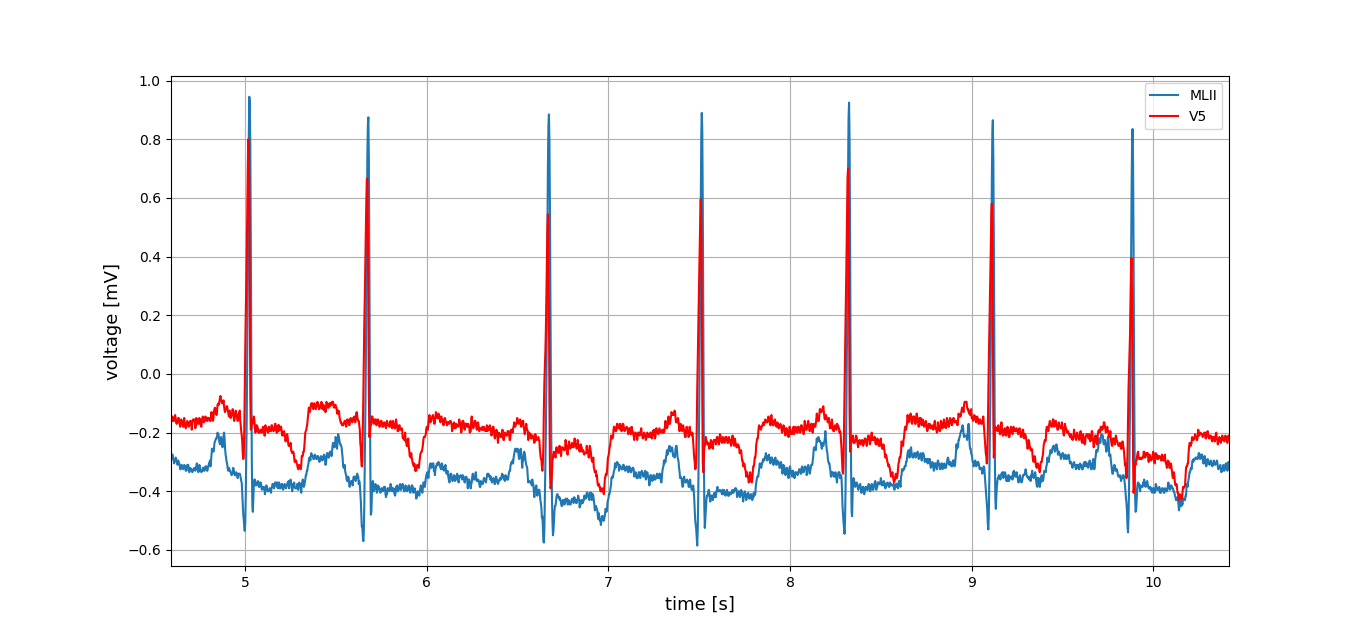
\includegraphics[width=15cm,height=12cm,keepaspectratio=true]{images/all_signals}
	\caption{
		The ECG signals from MIT-BIH dataset.
	}
	\label{fig:all_signals}
\end{figure}


The signals are in a raw form and need to be processed before they can be used. Most of the time, the signals are also contaminated with noise, baseline drift, etc. and they are required to be cleaned to get the correct values. 


\section{Preprocessing}
The ECG signal is required to be processed before it is analyzed, as it contains several noises and artifacts. The most common noises are the baseline wander and 60Hz power interference. Baseline wander generally appears because of the subject respiration or the body movements. It has a frequency range of 0Hz to 0.5Hz. The power interference affects the signals because of the electrical appliances in the surrounding.

Two different methods have been used to remove the noise and artifacts from the signal in the system implementation.

\begin{enumerate}
	\item Wavelet Transform Method
	\item Band-pass Filter Method
\end{enumerate}

\begin{figure}[h]
	\centering
	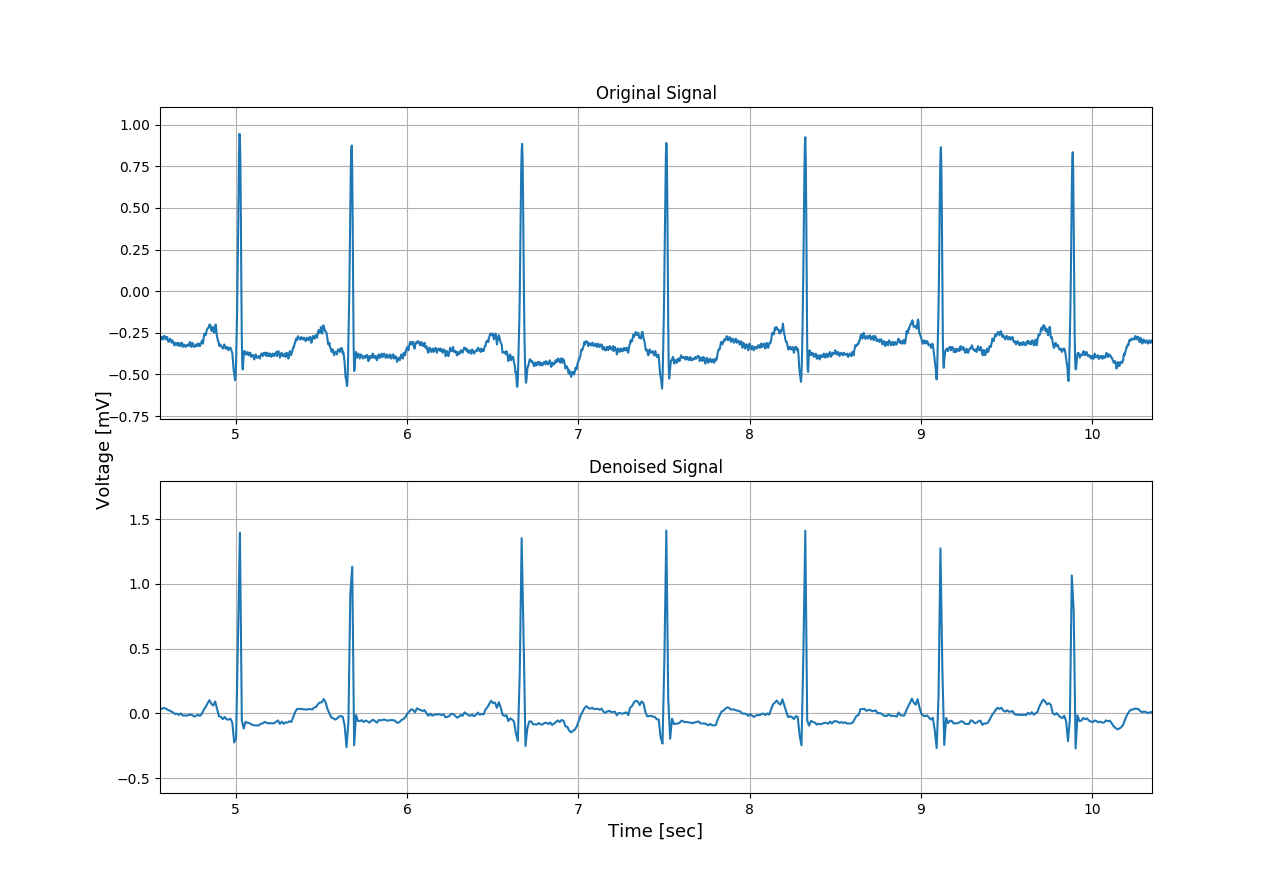
\includegraphics[width=15cm,height=12cm,keepaspectratio=true]{images/wavelet_denoised_1}
	\caption{
		The filtered ECG signal using wavelet.
	}
	\label{fig:wavelet_denoised}
\end{figure}


\subsection{Wavelet Transform Method}

The wavelet transform is a very interesting technique for analyzing the signal in the time-frequency domain. It distributes the signal in such a way that the resulting block is well localized in both time and frequency. Decomposition of the signal into different frequency bands is obtained by passing the signal through high-pass and low-pass filter respectively, which results in 2 sets of coefficients namely, approximation coefficients and detail coefficients. The approximation coefficients contain the low-pass filter output and the detail coefficients contain the high-pass filter output. The next step split the approximation coefficients again into 2 parts using the same process and so on.

The original signal contains the high-frequency noise and the baseline drift. The wavelet transform can be used to remove the corresponding noises and the baseline drift. The process starts by decomposing the original signal into 8 layers using wavelet type bior2.6, which results in the corresponding detail and approximation coefficients. Mostly, the layers 1 and 2 of the detail coefficients contain the high-frequency noise and the layer 8 of the approximation coefficients contain the baseline drift. Therefore, the layers 1 and 2 of the detail coefficients and layer 8 of the approximation coefficients are set to 0; which then results in the de-noised signal with no baseline drift. The resulting ECG signal can be seen in the Figure \ref{fig:wavelet_denoised}. 




\subsection{Band-pass Filter Method}
A band-pass filter is a type of filter which passes frequencies only in a certain range or spread without disturbing the input signal. The range of frequencies, let say, f1 and f2, are called the frequency passband.

A band-pass filter can be used to reduce the baseline drift, motion artifacts and high-frequency noise from the ECG signal. A passband of 3 Hz to 45 Hz has been used. After passing the ECG signal through the band-pass filter, the resulting signal produced is the de-noised signal with no high-frequency and baseline drift. The de-noised signal can be seen in the Figure \ref{fig:bandpass_denoised}. 

\begin{figure}[h]
	\centering
	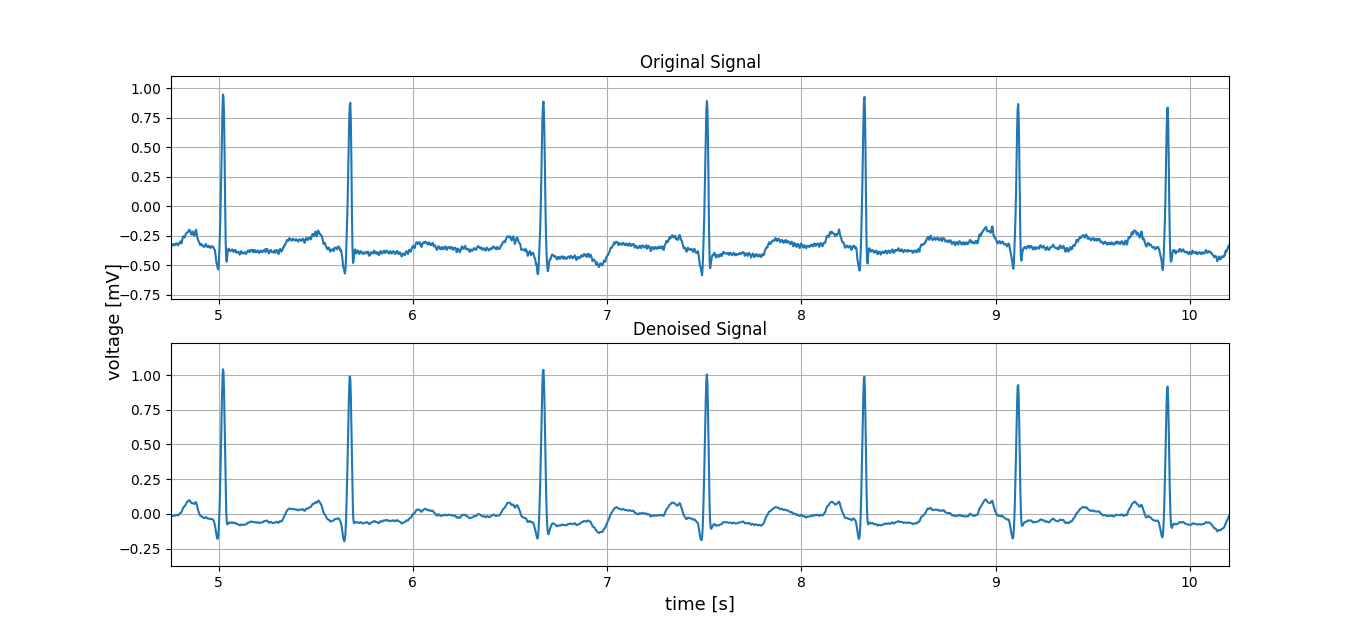
\includegraphics[width=15cm,height=12cm,keepaspectratio=true]{images/bandpass_denoised_1}
	\caption{
		The filtered ECG signal using bandpass filter.
	}
	\label{fig:bandpass_denoised}
\end{figure}


\renewcommand{\arraystretch}{2}
\begin{table}
	\caption{Wavelet Transform ECG Signal Frequency Range, taken from \cite{shang2014qrs}.} \label{tab:qrsenergy}
	
	\begin{center}
		\begin{tabular}{ | l | r | }
			\hline
			Transform Scale & Frequency Range (Hz) \\ \hline
			${2^1}$  & 90.0{\raise.17ex\hbox{$\scriptstyle\sim$}}180.0 \\ \hline
			${2^2}$  & 29.92{\raise.17ex\hbox{$\scriptstyle\sim$}}84.24  \\ \hline
			${2^3}$  & 1.52{\raise.17ex\hbox{$\scriptstyle\sim$}}38.88  \\ \hline
			${2^4}$  & 5.76{\raise.17ex\hbox{$\scriptstyle\sim$}}19.44  \\ 
			\hline
		\end{tabular}
	\end{center}
	
\end{table}


\section{QRS Detection}\label{sec:ecg_det}
QRS detection is the basis for processing the ECG signal. Regardless of what application is required, the accurate detection of QRS is a pre-requisite for feature extraction. A good wavelet base can help detect the features of ECG signal more appropriately with speed and accuracy. Therefore, Biorthogonal spline wavelet is used to detect QRS wave. Biorthogonal spline wavelet transform of ECG signal is calculated using the Mallat algorithm. Figure ~\ref{fig:detail_coefficients} shows the Biorthogonal spline wavelet transform of ECG signal at 4 different scales.

\begin{figure}[htpb]
	\centering
	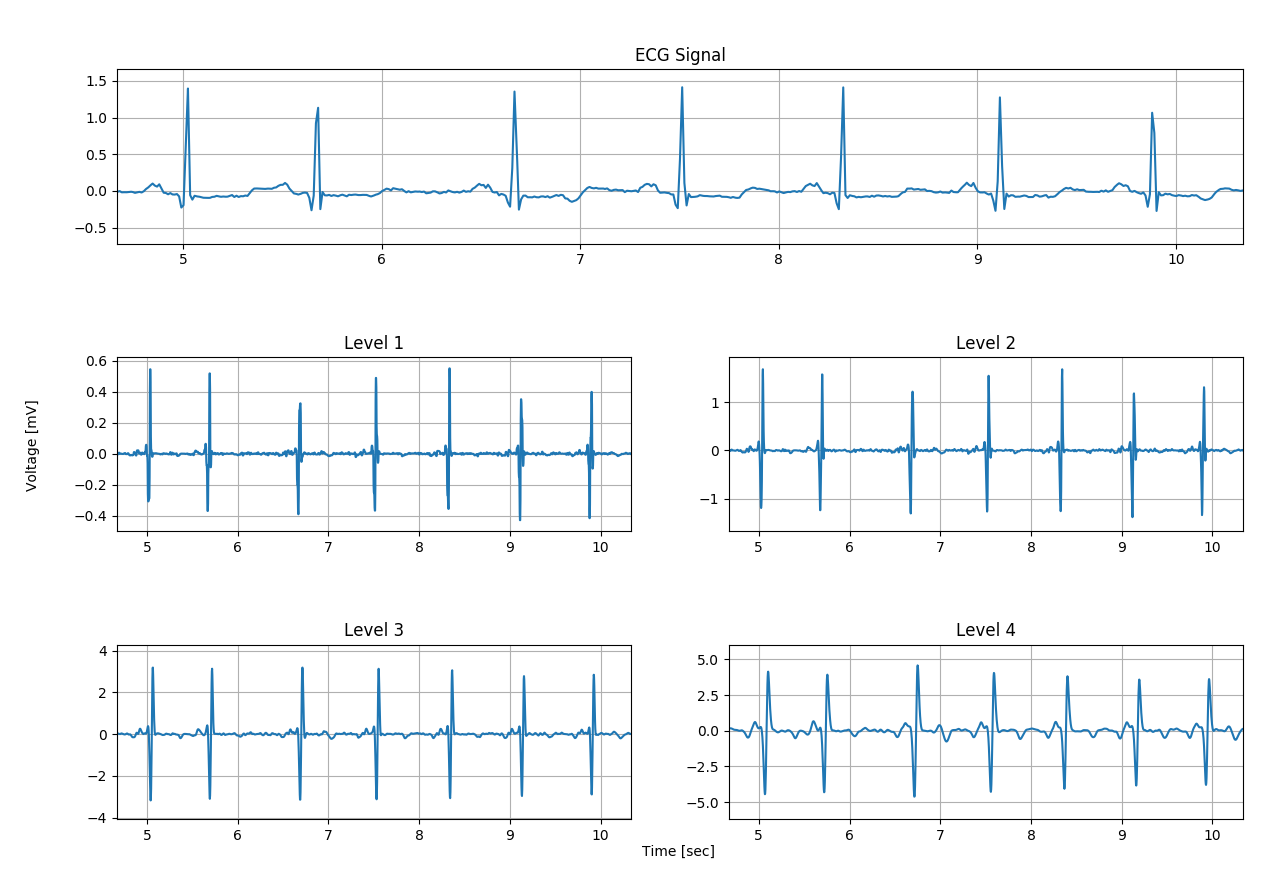
\includegraphics[width=17cm,height=17cm,keepaspectratio=true]{images/detail_coefficients}
	\caption{
		ECG signal and its decomposition at different scales.
	}
	\label{fig:detail_coefficients}
\end{figure}

Most of the QRS complex energy lies in the 3rd scale as can be seen in Table \ref{tab:qrsenergy}, therefore, the maximal minimal method can be used on the 3rd layer of the detail coefficient to find the R waves.  The process starts by taking the first derivative of the 3rd layer to find the maximum and minimum points and then the 2nd derivative to locate the actual maximum and minimum values. The resulting waves are shown in Figure \ref{fig:maximas_on_level_3}. As it can be seen that, there are other peaks available as well, therefore, to get the maximum and minimum pair only, a threshold needs to be set. And all the values that do not fulfill the threshold should be discarded. 
For finding the threshold, the result of the 2nd derivative is divided into 4 parts and from each part, the maximum value is located. After getting the values, the average is calculated for these values and that average is then divided by 3. The resultant value is a new threshold. The pair can be seen in Figure \ref{fig:max_pair}.

\begin{figure}[htpb]
	\centering
	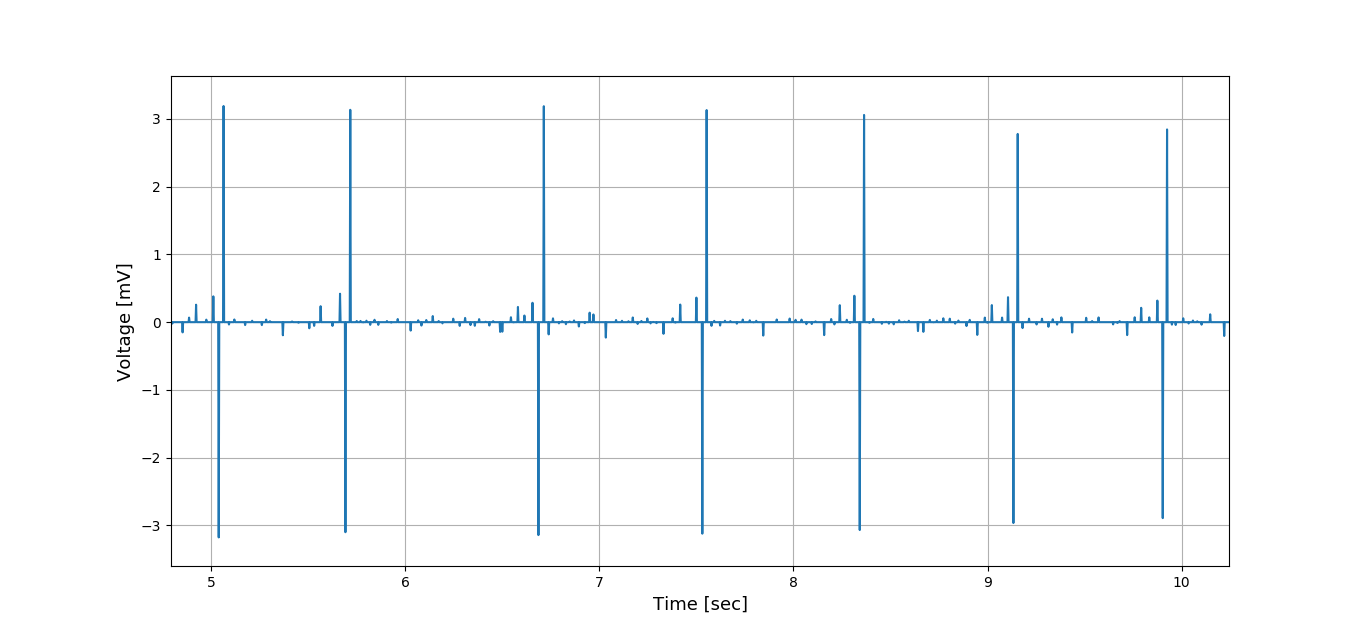
\includegraphics[width=15cm,height=15cm,keepaspectratio=true]{images/maximas_on_level_3}
	\caption{
		Maximum and minimum values on scale 3.
	}
	\label{fig:maximas_on_level_3}
\end{figure}

\begin{figure}[htpb]
	\centering
	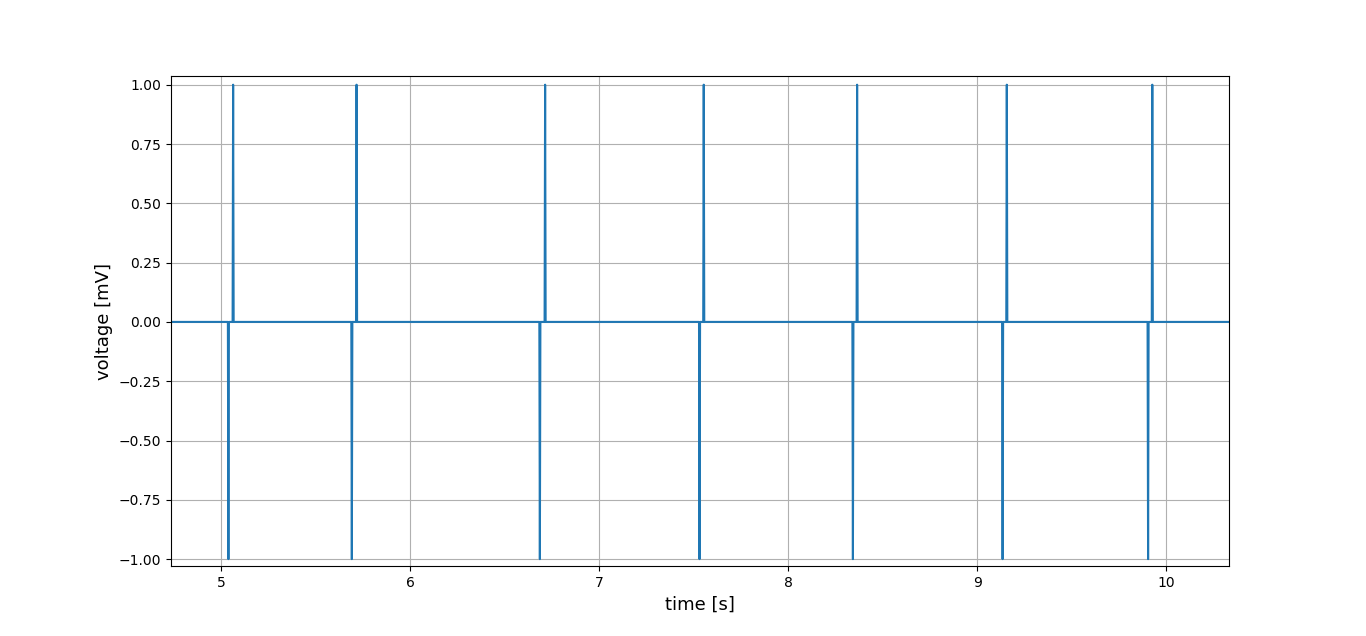
\includegraphics[width=15cm,height=12cm,keepaspectratio=true]{images/max_pair}
	\caption{
		Maximum and minimum values pair for finding the R peaks.
	}
	\label{fig:max_pair}
\end{figure}

The value of R wave lies at the zero-crossing point (with a little delay) which is between the maximum and the minimum value pair. For compensating the delay, a maximum value can be searched in the window of 20 points to the zero-crossing point. The detected R-peaks can be seen in Figure \ref{fig:r_peaks}. The flow chart for finding the R peaks is shown in figure \ref{fig:r_peaks_flow_chart}.

\begin{figure}[htpb]
	\centering
	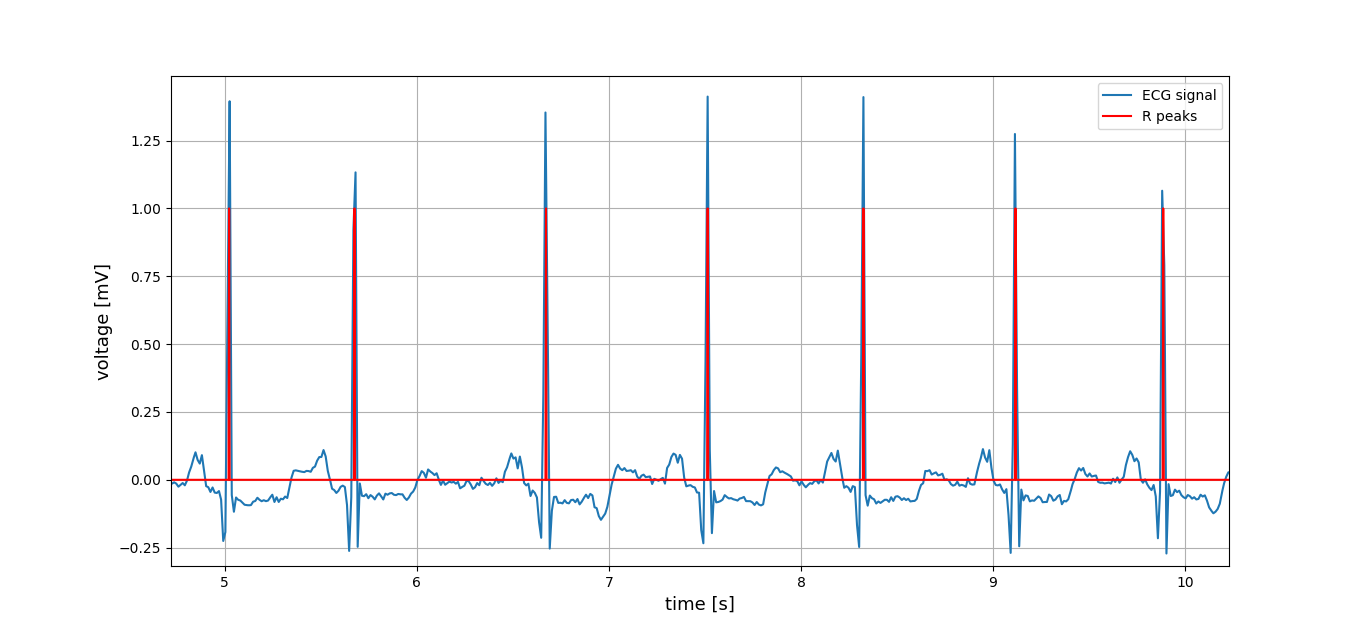
\includegraphics[width=15cm,height=15cm,keepaspectratio=true]{images/r_peaks}
	\caption{
		Detected R peaks.
	}
	\label{fig:r_peaks}
\end{figure}


\begin{figure}[htpb]
	\centering
	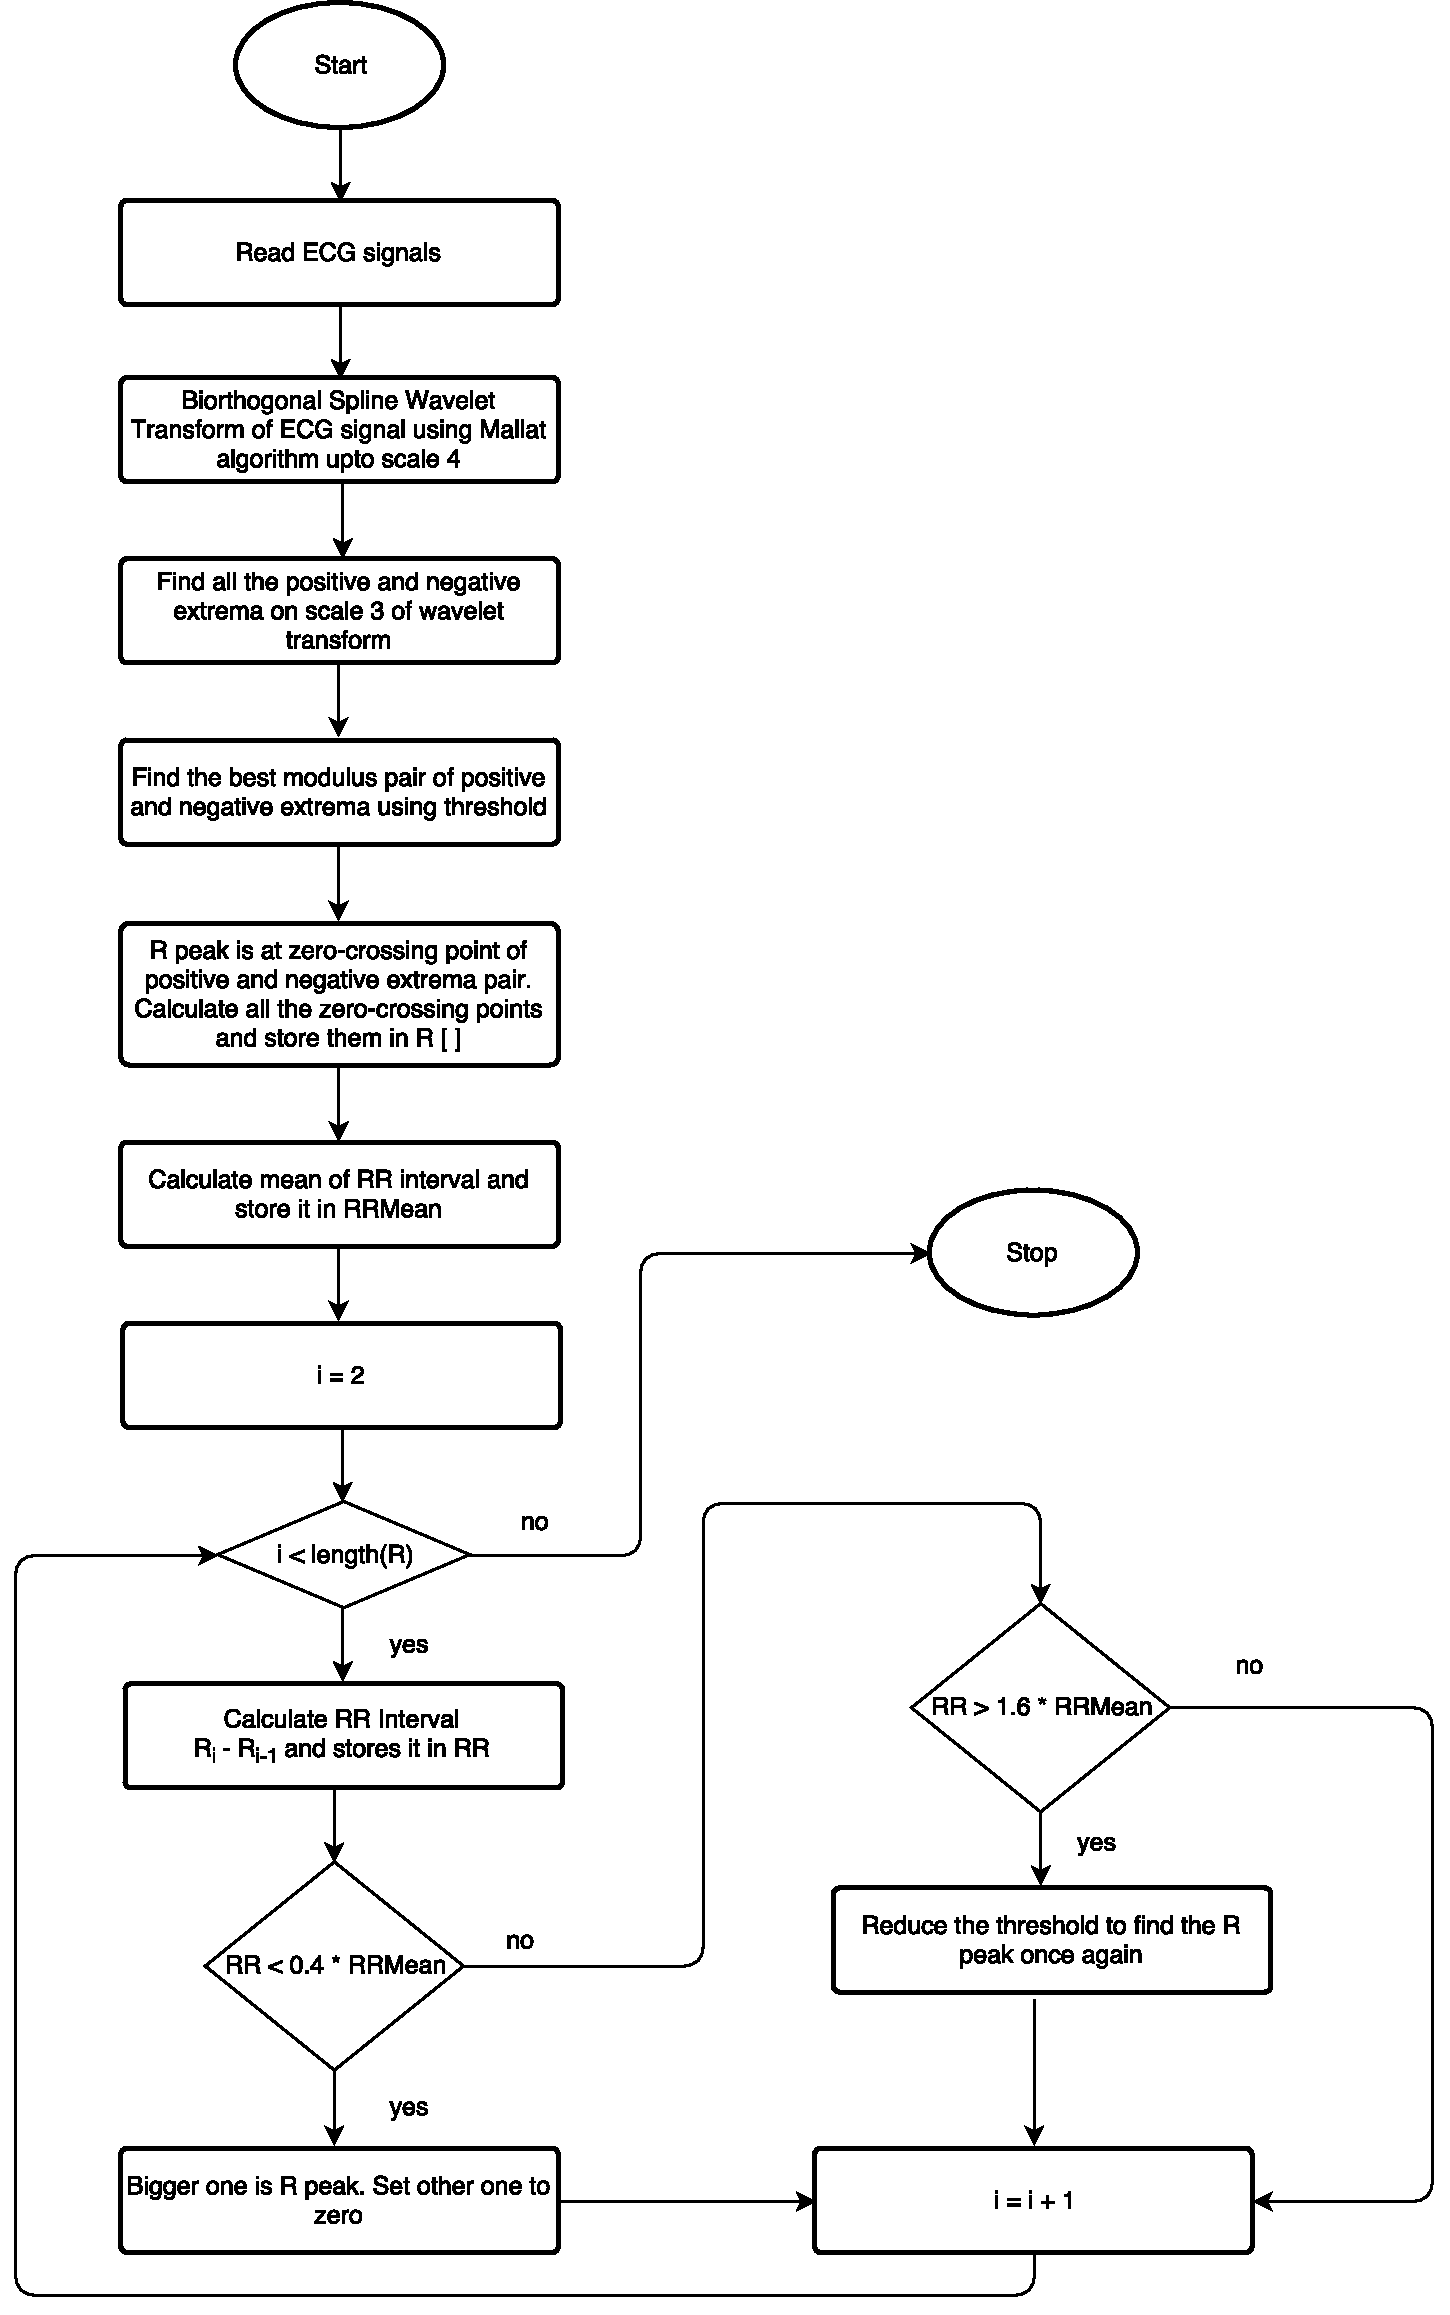
\includegraphics[width=25cm,height=22cm,keepaspectratio=true]{images/qrs.pdf}
	\caption{
		R peak flow chart.
	}
	\label{fig:r_peaks_flow_chart}
\end{figure}



After getting the R-peaks, Q and S peaks have to be detected. Q and S wave generally are of high frequency; therefore, their energies are mainly on the 1st scale. For finding the Q wave, the algorithm starts by looking on the left side of the R wave and finds the first non-zero value i.e. the Q wave. And because of the delay, the minimum value is searched in the window of 10 points to the detected Q wave. The same process is executed for the S wave, but in this case, the direction was on the right side of the R wave. The detected QRS complex can be seen in Figure \ref{fig:qrs_peaks}.

\begin{figure}[htpb]
	\centering
	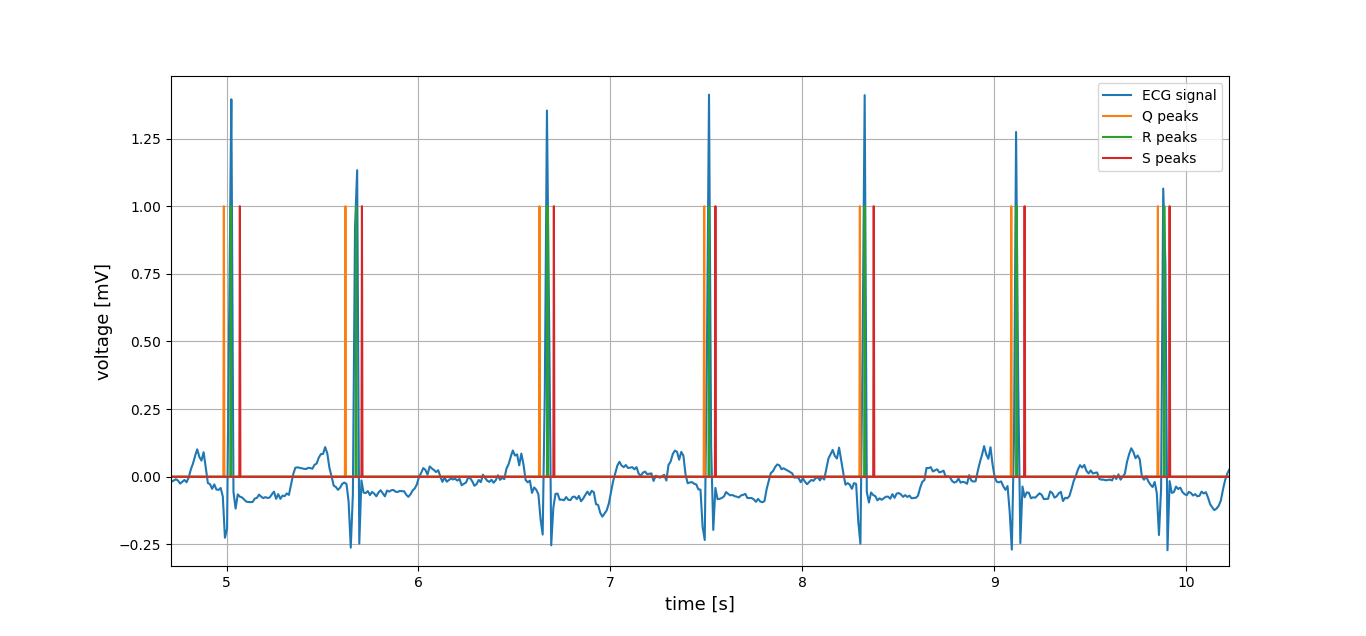
\includegraphics[width=15cm,height=15cm,keepaspectratio=true]{images/qrs}
	\caption{
		Detected Q, R and S peaks.
	}
	\label{fig:qrs_peaks}
\end{figure}


\begin{figure}[htpb]
	\centering
	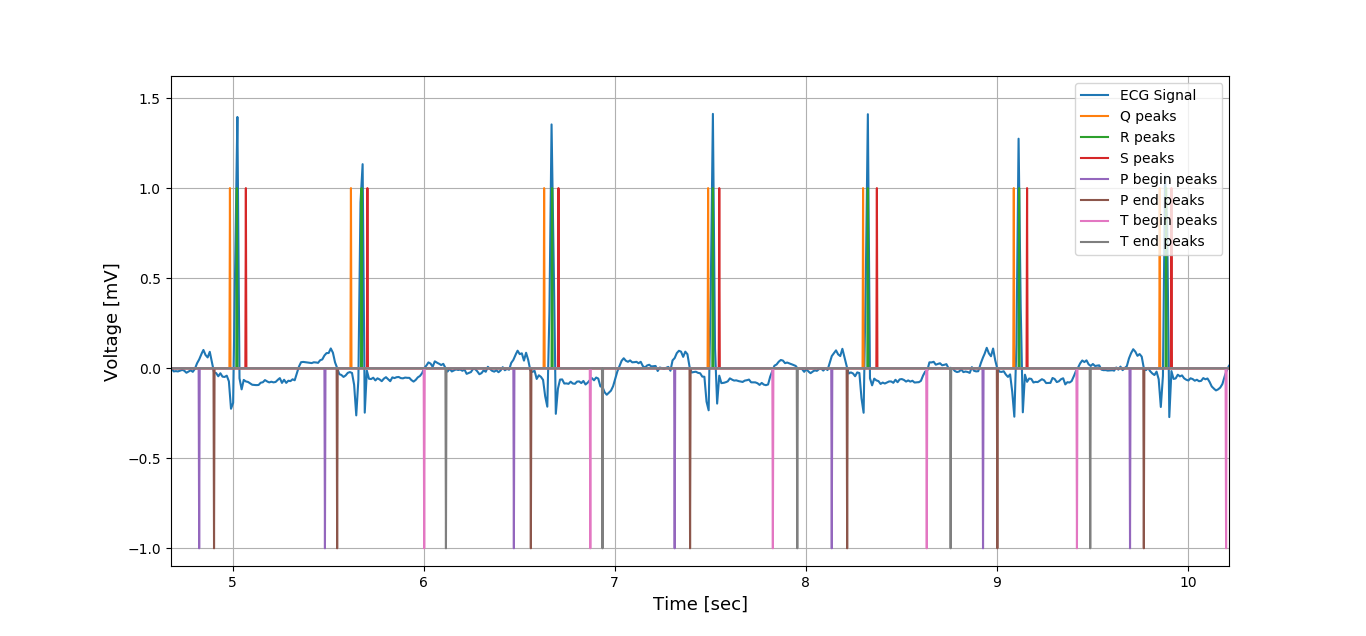
\includegraphics[width=15cm,height=15cm,keepaspectratio=true]{images/pqrst}
	\caption{
		Detected P,Q,R,S and T waves.
	}
	\label{fig:pqrst}
\end{figure}



\begin{figure}[htpb]
	\centering
	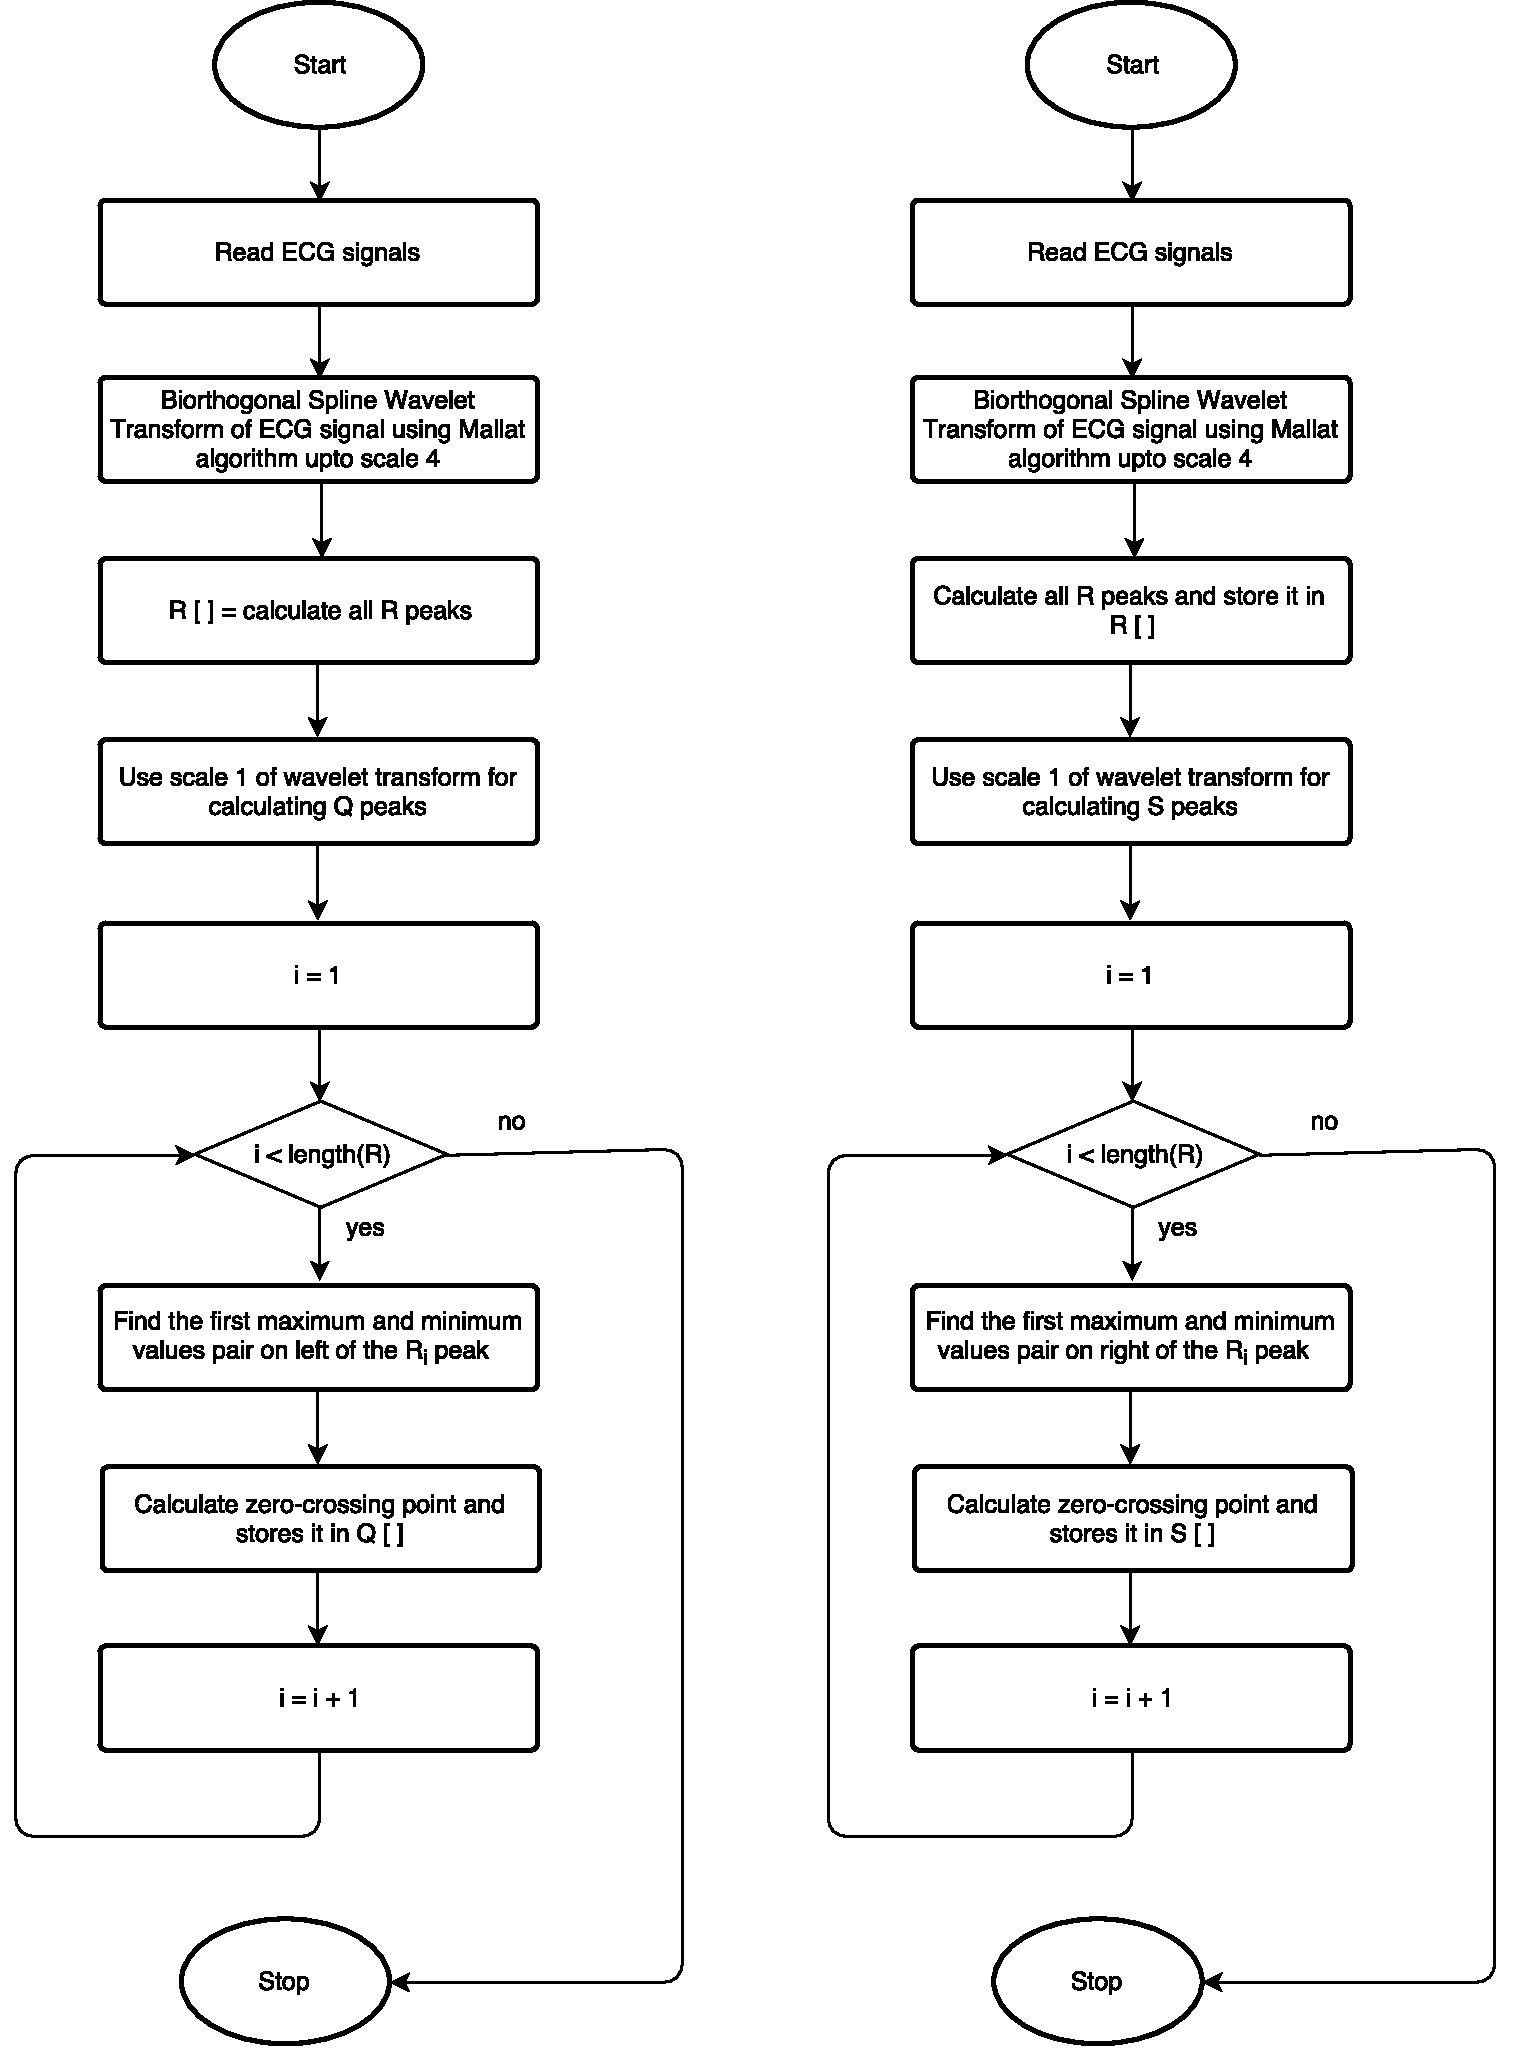
\includegraphics[width=25cm,height=22cm,keepaspectratio=true]{images/q-and-s.pdf}
	\caption{
		Q and S peak flow chart.
	}
	\label{fig:qs}
\end{figure}



After detecting the QRS complex, P and T waves are required to be detected as they also have very important significance to identify the arrhythmia. P wave generally occurred before the QRS complex and T wave after the QRS complex, therefore, they can be detected based on QRS location.

\section{P and T Wave Detection}
Most of the P and T waves energy lies on the scale 4 and the QRS complex energy lies on the scale 3 of detail coefficient. If QRS complex (that was detected on scale 3) is used, it sometimes misses the P wave or identifies the wrong position. Therefore, it is first required to detect QRS complex on scale 4 and then find P and T waves. The same algorithm is used to detect the QRS complex on scale 4 that is used to detect on scale 3, as described in section \ref{sec:ecg_det}.

After getting the QRS on scale 4, a window size of 100 is used for detecting the P wave. The starting point of the window is one sample less than from Q wave position and if the window size is added to this position, we get the beginning of the window. RR interval is also calculated between the 2 consecutive R peaks. 1/3 of the RR interval is used for detecting the P wave and 2/3 of the RR interval is used for detecting the T wave. Once the window is identified on the scale 4, the max and min values are identified in that window as P wave lies on the zero-crossing point of min and max pair. The average is taken to calculate the P wave position of scale 4. Once the P wave position is calculated, the P wave is identified relatively on the original signal. One point to note here is that the scale 4 data is shifted because of filtering, therefore, it is required to shift the detected position few samples back to get the appropriate value.

The same approach is used for detecting the T wave, but instead of looking the window before the QRS complex, here the window is searched after the QRS complex for detecting the T wave.

All detected waves can be seen in the figure \ref{fig:pqrst}. The flow chart for finding the P wave and T wave is shown in figures \ref{fig:p_peaks_flow_chart} and \ref{fig:t_peaks_flow_chart} respectively.


\begin{figure}[htpb]
	\centering
	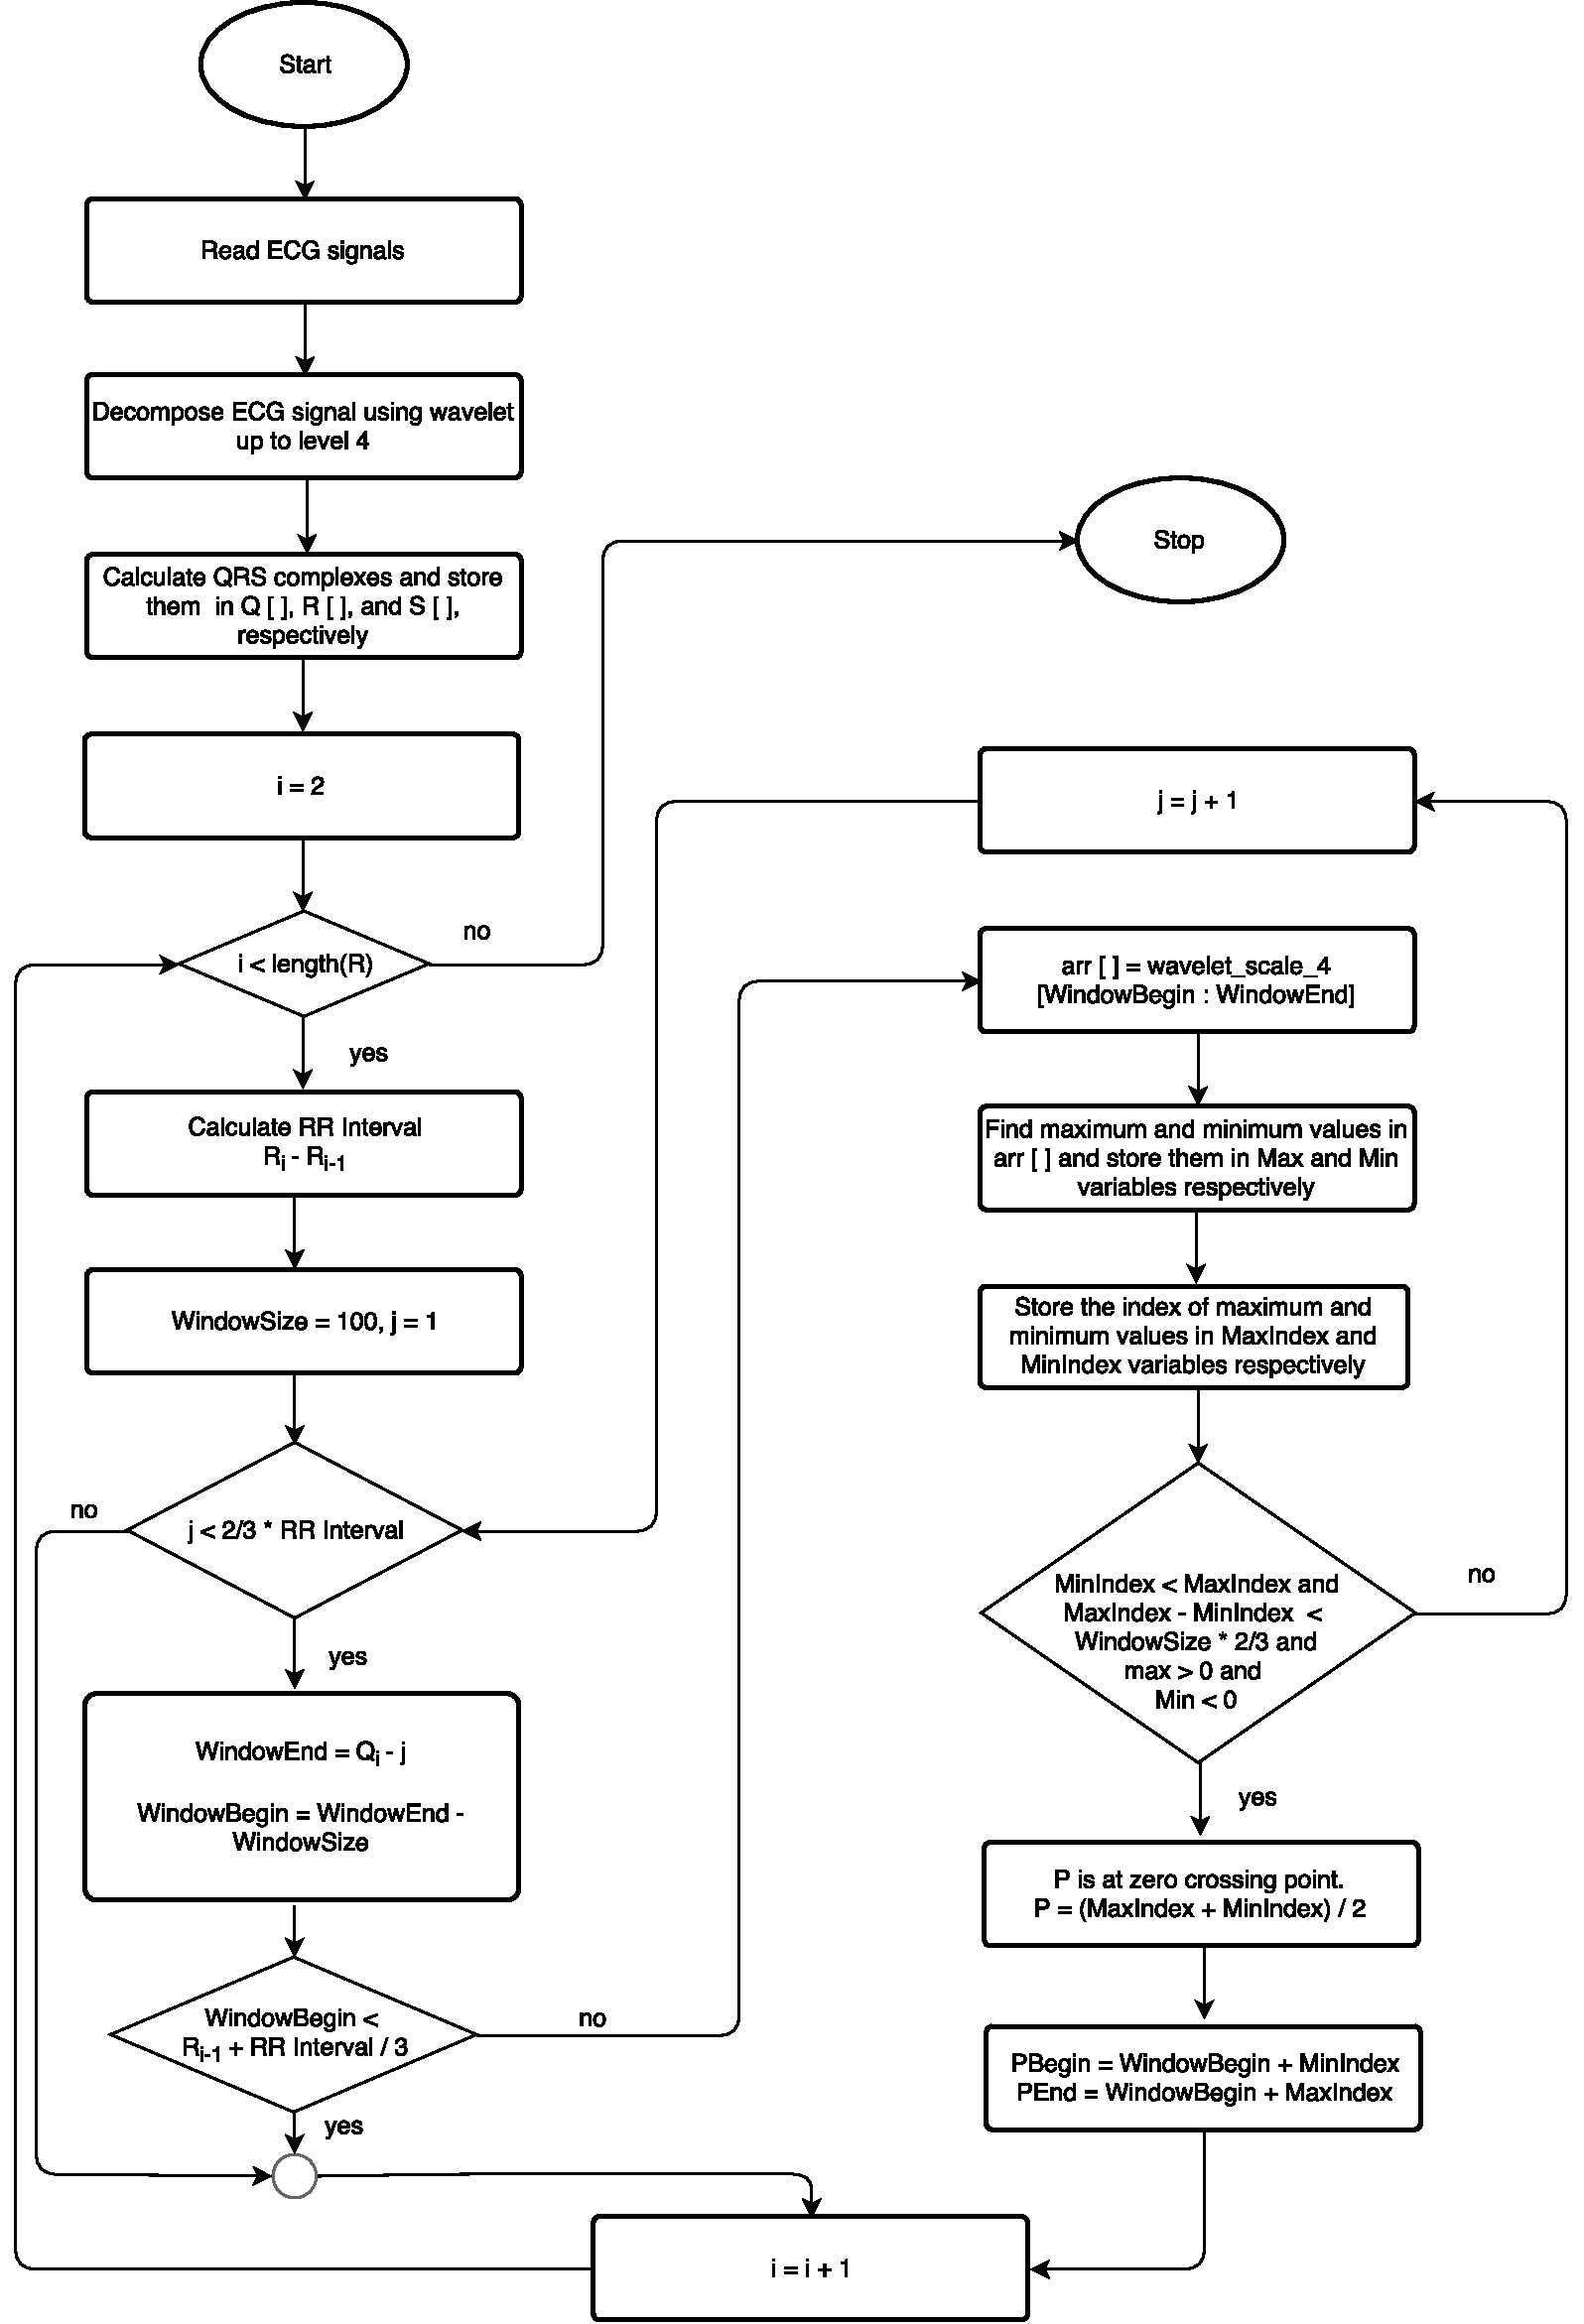
\includegraphics[width=25cm,height=22cm,keepaspectratio=true]{images/p_Wave.pdf}
	\caption{
		P wave flow chart.
	}
	\label{fig:p_peaks_flow_chart}
\end{figure}

\begin{figure}[htpb]
	\centering
	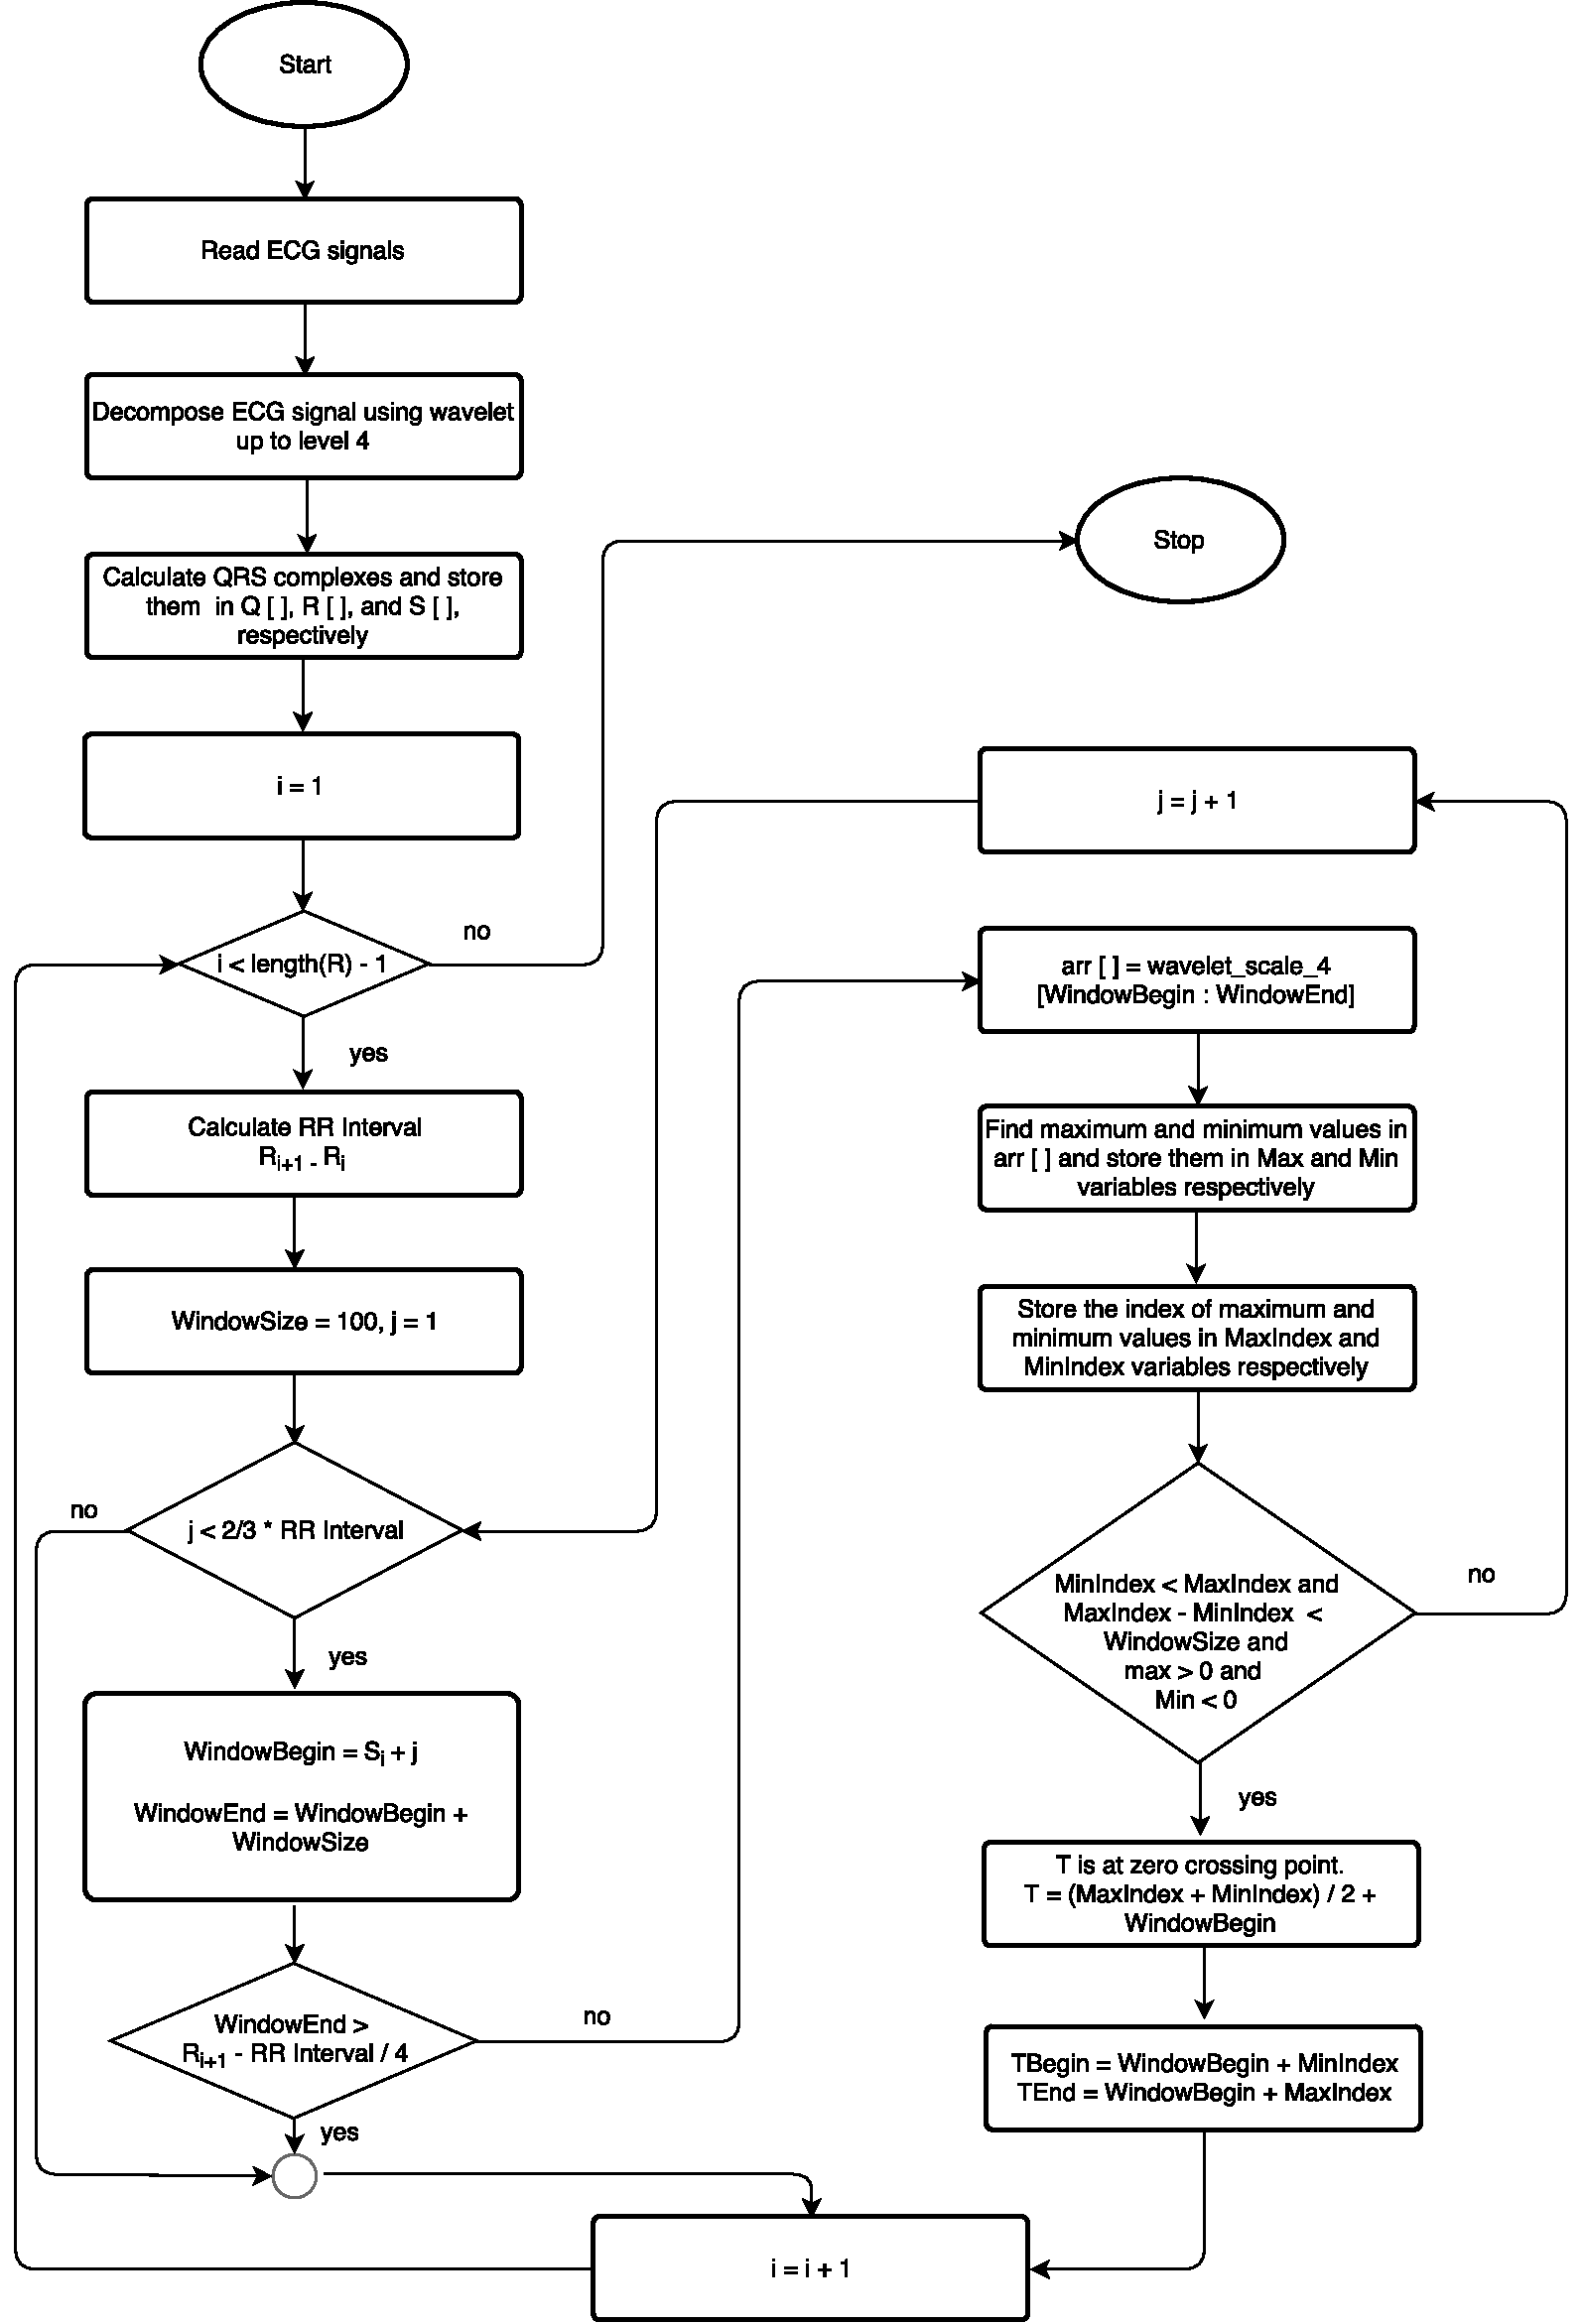
\includegraphics[width=25cm,height=22cm,keepaspectratio=true]{images/T_Wave.pdf}
	\caption{
		T wave flow chart.
	}
	\label{fig:t_peaks_flow_chart}
\end{figure}


\section{Heart Rate Calculation}
The heart rate is calculated by first counting the number of R peaks in a 10 seconds window and then multiply the count by 6 to get the heart rate.

\begin{center}
	$HeartRate = number\_of\_R\_peaks \times 6$
\end{center}

\section{Algorithm Execution on ECG Chair Data}
The data used in the development of ECG feature extraction algorithm is taken from MIT-BIH data set and the algorithm works great with that data set. To analyze the performance of algorithm on the ECG chair data that is used in the implementation of the system, the data is collected from the ECG chair and passed to the algorithm. It turns out that the algorithm works perfectly fine with this data as well. The original ECG signal can be seen in Figure \ref{fig:device_ecg_orignal} and the extracted features can be seen in Figure \ref{fig:device_ecg_feature_extraction}.

\begin{figure}[htpb]
	\centering
	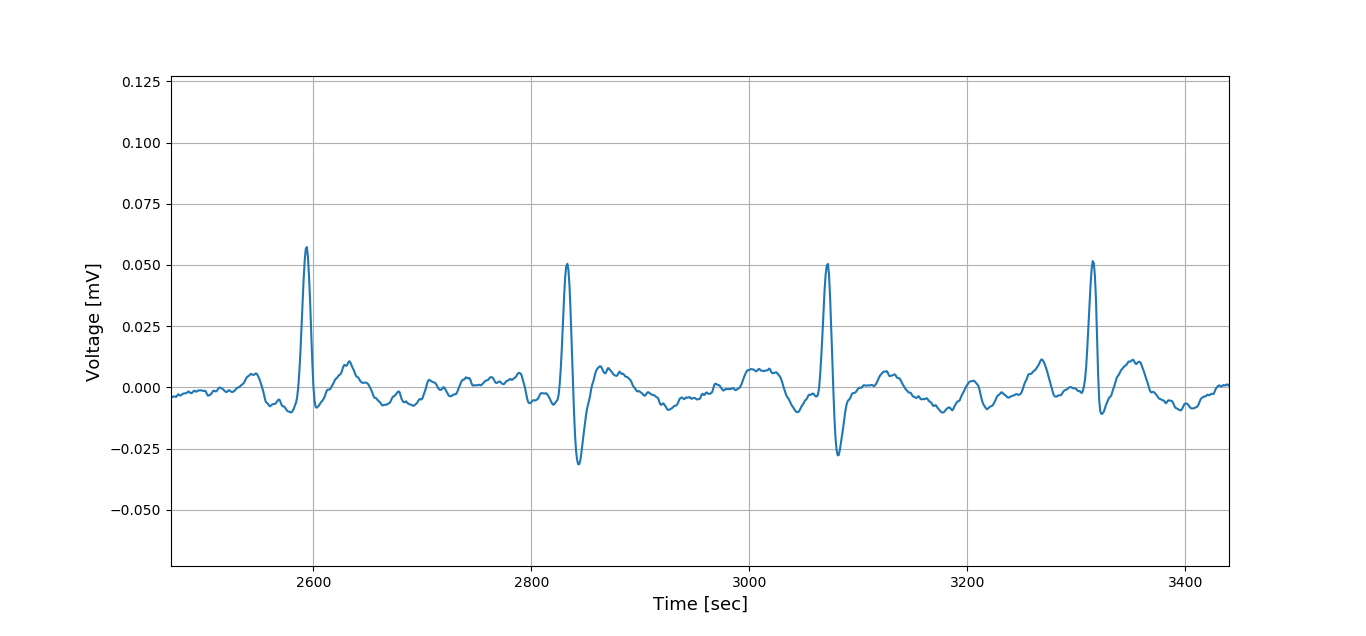
\includegraphics[width=15cm,height=15cm,keepaspectratio=true]{images/device_ecg_orignal}
	\caption{
		Original ECG chair signal.
	}
	\label{fig:device_ecg_orignal}
\end{figure}

\begin{figure}[htpb]
	\centering
	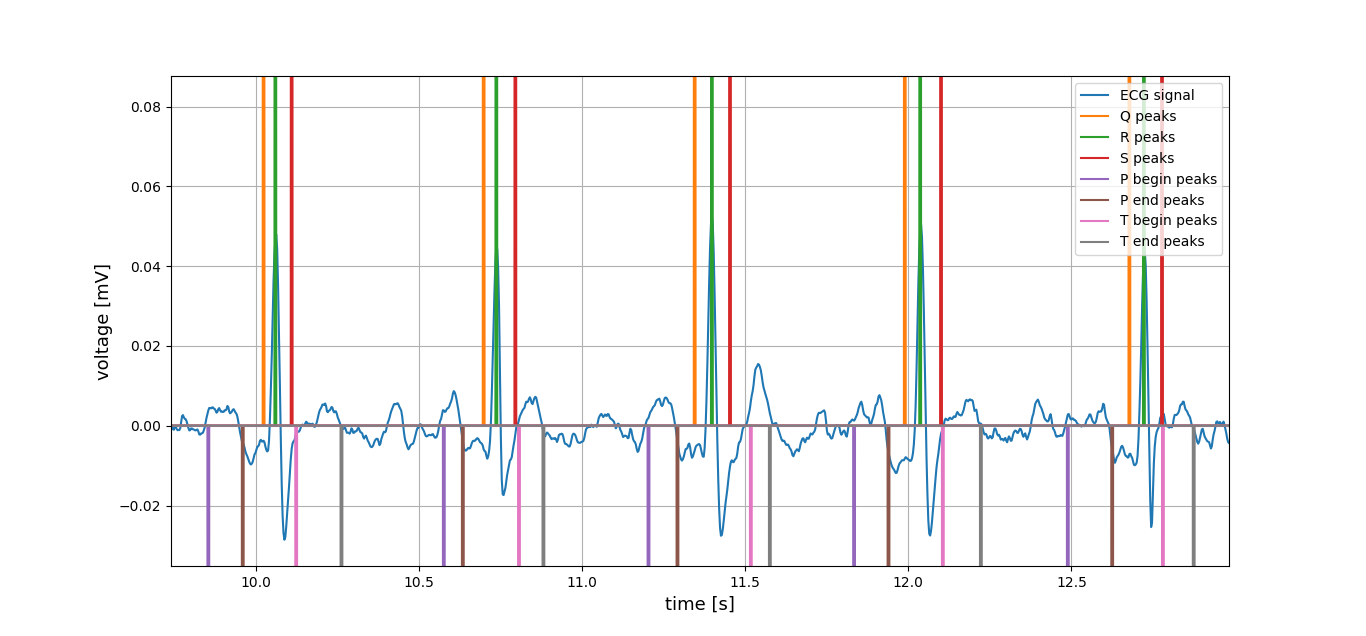
\includegraphics[width=15cm,height=15cm,keepaspectratio=true]{images/device_ecg_feature_extraction.png}
	\caption{
		Detected P,Q,R,S and T waves on the ECG chair signal.
	}
	\label{fig:device_ecg_feature_extraction}
\end{figure}
